\hypertarget{sec:introduction}{%
\section{Introduction}\label{sec:introduction}}

Chapter \ref{ch:intro} defined a \emph{responsive feature} as any
linguistic feature which is sensitive to the acquisition setting. In
particular, L2-difficult features are responsive in this sense: by
definition, such features pose a difficulty for, and only for, acquirers
beyond a critical age. The Trudgill conjecture (Chapter \ref{ch:george})
predicts that such features are prone to being lost if enough acquirers
beyond this critical age are found in the speech community. Writing on
simplification of adjective inflection in Bergen Norwegian, Trudgill
proposes:

\begin{quote}
My suggestion is that when the proportion of non-native becomes as close
to 50\% as this -- the proportion of non-native speakers of Norwegian in
Bergen was certainly very high (4,000 out of 9,000) -- the number of
face-to-face dialect-contact type interactions, and therefore potential
instances of accommodation {[}\ldots{]}, would have reached a threshold
level at which some aspects of the non-native variety could transfer to
the native \autocite[pp.~57--58]{Tru2011}.
\end{quote}

The present chapter undertakes a quantitative and computational
recapitulation of this proposal, asking just how many post-critical-age
acquirers must be present in the speech community for L2-difficult
features to be lost. If there indeed exists a threshold of
simplification due to the responsive nature of some or other feature,
what is this threshold? Fifty percent L2 learners? Sixty percent? Or
possibly a number whose precise value depends, in some way, on other
factors involved in the contact situation? Moreover, how long must the
contact situation continue for simplification to be permanent, so that
the L2-difficult feature is not simply restored once L2 learners are
removed from the population? Finally, how do sociodemographic factors
such as the frequency of interactions between L2 learners and L1
speakers affect the likelihood of simplification?

The challenges involved in answering these questions ought to be clear
from the outset. An empirical answer would require, at a minimum, a
sample of language histories some of which culminate in loss of an
L2-difficult feature, with others culminating in its retention, together
with reliable estimates of the likely numbers of post-critical-age
acquirers in each case, combined with information about further factors
such as the degree of L2-difficulty exhibited by the feature in
question, the duration for which L2 learning was in place, and the
frequencies of different patterns of interaction between the different
subpopulations. It is clear that empirical data are not available to
this extent, at this resolution, in most cases of interest. As a
consequence, a mixed methodology, combining empirical data, theory, and
modelling, is called for.

The strategy adopted in the present chapter is to draw upon the
predictive power of mechanistic modelling \autocite{GeritzKisdi2012}. It
is first demonstrated how feature responsivity can be captured in a
simple stochastic model of language acquisition. A mixed population is
then introduced, one in which some learners acquire the language before
the critical age, the remaining being post-critical-age acquirers; for
ease of exposition, I will refer to the former as L1 learners, and the
latter as L2 learners, in what follows.\footnote{It is important to bear
  in mind that, with this nomenclature, our L2 learners do not comprise
  individuals who exhibit childhood bilingualism -- such individuals
  learn an L2 but learn it before the critical age and hence the
  responsive features do not respond in their case. Moreover, empirical
  reality accommodates for more nuance than can be captured by a
  strictly binary cutoff between pre-critical age and post-critical age.
  See Chapter \ref{ch:george} for more discussion of these points.} As
these learners interact, the frequency of the L2-difficult feature may
go up or down in the population; we are chiefly interested in the
question of under what circumstances this frequency vanishes to zero,
corresponding to full simplification.

The chapter builds upon work published in \textcite{Kauhanen2022}. In
that article, the above questions were answered in a particular limiting
case of the model, known as the deterministic limit. This special case
is characterized by the following idealizing assumptions: (i) there are
infinitely many learners in each group (L1 and L2), (ii) learners pick
interlocutors entirely at random, and (iii) all learners within a group
behave the same. For completeness, the results of the earlier paper are
restated and discussed below (in Section
\ref{sec:bifurcation-threshold}). The present chapter ventures beyond
the deterministic limit, exploring a number of empirically relevant
scenarios of the full stochastic model in computer simulations. A
methodological innovation -- efficient simulation of large populations
through the use of a Beta approximation to describe the statistical
equilibrium of language learning -- is also introduced and discussed.

The results demonstrate that the stochastic simulations are broadly in
line with the deterministic prediction, up to very slight overestimation
of the likelihood of contact-induced simplification by the latter due to
the fundamental well-mixing assumption of the deterministic-limit model.
Simulations involving systematic sweeps across the model's parameter
space uncover further, more fine-grained results, such as the (prima
facie counterintuitive) fact that simplification is supported by
population structures in which interactions between the L1 and L2
learner subpopulations are less frequent than interactions within
subpopulations. Finally, two detailed simulation case studies, one on
the expression of subjects in Afro-Peruvian Spanish, the other on the
loss of verbal morphology in Afrikaans, support the claims that were
made, based on the deterministic limit, in \textcite{Kauhanen2022}.

\hypertarget{sec:responsive-features}{%
\section{Responsive features in language
acquisition}\label{sec:responsive-features}}

Throughout this chapter, it is assumed that language learners need to
decide between two grammars, one (and only one) of which carries a
responsive feature.\footnote{These assumptions are made in order to keep
  the model simple, without losing the essential intuition of
  competition between a responsive grammar and a non-responsive one. It
  would be relatively straightforward to generalize the model for
  multiple competing grammars, each of which may involve some
  (potentially non-zero) amount of L2-difficulty. This and other
  potential avenues for further research are discussed at more length in
  Section \ref{sec:discussion}.} I will denote the L2-difficult grammar
with \(G_1\) and its competitor with \(G_2\). The grammars accept
languages \(L_1\) and \(L_2\), respectively, understood as sets of
well-formed strings, constructed out of a common alphabet. In general,
\(L_1\) and \(L_2\) may overlap; cf.~Figure \ref{fig:venn}. The symbol
\(a_1\) will be used to denote the probability of someone employing
\(G_1\) producing a string belonging to the set \(L_1 \setminus L_2\)
(i.e.~a string that \(G_2\) does not accept), and similarly \(a_2\) will
be used for the probability of someone employing \(G_2\) producing a
string in \(L_2 \setminus L_1\). These quantities will be referred to as
the \emph{advantages} of the two grammars in what follows.\footnote{In
  Chapter \ref{ch:raquel}, where competition between more than two
  grammars is considered, these pairwise advantages are denoted
  \(a_{21}\) and \(a_{12}\).} They are also assumed to reflect the weak
generative capacities of the two grammars \autocite[cf.][]{Yang2000} and
may thus be assumed to be constant within any given competition
situation.

\begin{figure}
\hypertarget{fig:venn}{%
\centering
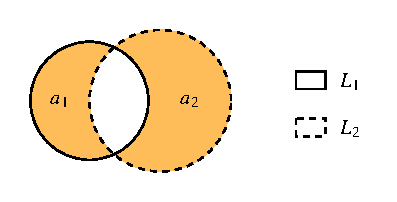
\includegraphics[width=0.6\textwidth]{figures/ch5/venn.pdf}
\caption{Two grammars, \(G_1\) and \(G_2\), generate languages \(L_1\)
and \(L_2\), represented here as intersecting sets. The shaded areas are
the sets \(L_1 \setminus L_2\) and \(L_2 \setminus L_1\); their sizes
represent the probabilities that strings from these sets are produced,
\(a_1\) and \(a_2\) (referred to as the advantages of \(G_1\) and
\(G_2\), respectively).}\label{fig:venn}
}
\end{figure}

Each language user is assumed to embody a pair of \emph{weights} for the
two grammars; formally, these weights constitute a categorical
probability distribution over the grammars. The weight of \(G_1\) will
be denoted \(W_1\) and the weight of \(G_2\) with \(W_2 = 1 - W_1\);
these are random variables whose values change in response to the
linguistic input received by the language user or learner. These changes
could in principle be implemented by any number of imaginable
mechanisms, and it is one of the goals of language acquisition and
learnability research to disentangle probable from improbable mechanisms
of learning. In order to obtain a reasonably tractable mathematical
model, I follow the variational learning framework of
\textcite{Yang2002}, itself founded upon the pioneering work of
\textcite{BushMosteller1955} on general statistical mechanisms of
reinforcement.

Let us first outline how the learning algorithm works for an acquirer
under the critical age. Upon receiving an input sequence
\(s \in L_1 \cup L_2\), the learner chooses one of the two grammars to
use: \(G_1\) with probability \(W_1\), and \(G_2\) with probability
\(W_2\). The learner then attempts to parse the input sequence. If the
chosen grammar accepts the input, this grammar's weight is increased and
the weight of its competitor is decreased. If the grammar does not
accept the input, the reverse operation is carried out, decreasing this
grammar's weight and increasing the competitor's weight.

Concretely, the changes made to the weights follow the linear
reward--penalty scheme of \textcite{BushMosteller1955}. The mathematics
of this are summarized in Table \ref{tbl-BM}, from which the updates to
\(W_1\) and \(W_2\) can be read under all possible circumstances. The
number \(\gamma\) is a learning rate parameter which regulates the
magnitude of the updates the learner makes to the weight distribution;
this parameter must satisfy the technical requirement
\(0 < \gamma < 1\).\footnote{Technically, \(\gamma = 1\) is also
  possible, leading to a model in which learners ``hop'' categorically
  between \(G_1\) and \(G_2\) \autocites[cf.][]{GibWex1994,NiyBer1996}.
  I leave this special case aside here.}

\begin{table}
\caption{Learning algorithm for L1 learner \parencite{BushMosteller1955,Yang2002}. The new values of $W_1$ and $W_2$ are $W_1' = W_1 + \Delta W_1$ and $W_2' = W_2 + \Delta W_2$. A positive $\Delta W_1$ (resp. $\Delta W_2$) rewards $G_1$ (resp. $G_2$), while a negative value punishes it.}\label{tbl-BM}

\begin{tabular}{cccc}
\toprule
Input string & Grammar chosen & $\Delta W_1$ (update to $W_1$) & $\Delta W_2$ (update to $W_2$) \\
\midrule
$s \in L_1 \setminus L_2$  & $G_1$          & $\gamma W_2$           & $-\gamma W_2$ \\
$s \in L_1 \setminus L_2$  & $G_2$          & $\gamma W_2$ & $-\gamma W_2$ \\
$s \in L_1 \cap L_2$ & $G_1$ & $\gamma W_2$ & $-\gamma W_2$ \\
$s \in L_1 \cap L_2$ & $G_2$ & $ - \gamma W_1$ & $\gamma W_1$ \\
$s \in L_2 \setminus L_1$ & $G_1$ & $- \gamma W_1$ & $\gamma W_1$ \\
$s \in L_2 \setminus L_1$ & $G_2$ & $- \gamma W_1$ & $\gamma W_1$ \\
\bottomrule
\end{tabular}
\end{table}

\begin{table}
\caption{Learning algorithm for L2 learner \parencite{Kauhanen2022}. The new values of $W_1$ and $W_2$ are $W_1' = W_1 + \Delta W_1$ and $W_2' = W_2 + \Delta W_2$.}\label{tbl-BM2}

\begin{tabular}{cccc}
\toprule
Input string & Grammar chosen & $\Delta W_1$ (update to $W_1$) & $\Delta W_2$ (update to $W_2$) \\
\midrule
$s \in L_1 \setminus L_2$  & $G_1$          & $\gamma W_2 - \delta W_1$           & $-\gamma W_2 + \delta W_1$ \\
$s \in L_1 \setminus L_2$  & $G_2$          & $\gamma W_2 - \delta W_1$ & $-\gamma W_2 + \delta W_1$ \\
$s \in L_1 \cap L_2$ & $G_1$ & $\gamma W_2 - \delta W_1$ & $-\gamma W_2 + \delta W_1$ \\
$s \in L_1 \cap L_2$ & $G_2$ & $- \gamma W_1 - \delta W_1$ & $\gamma W_1 + \delta W_1$ \\
$s \in L_2 \setminus L_1$ & $G_1$ & $- \gamma W_1 - \delta W_1$ & $\gamma W_1 + \delta W_1$ \\
$s \in L_2 \setminus L_1$ & $G_2$ & $- \gamma W_1 - \delta W_1$ & $\gamma W_1 + \delta W_1$ \\
\bottomrule
\end{tabular}
\end{table}

To model feature responsivity, \textcite{Kauhanen2022} introduced a
simple modification to this basic algorithm. For a learner past the
critical age, a second learning rate parameter \(\delta\) is introduced
whose effect is to render the acquisition of \(G_1\) more difficult for
the learner.\footnote{To ensure \(W_1\) and \(W_2\) always remain
  probabilities, a technical requirement is that
  \(0 < \delta < 1 - \gamma\).} The update rule is given in Table
\ref{tbl-BM2}. It is obvious that, under this modification of the
algorithm, grammar \(G_1\) faces an inherent disadvantage compared to
grammar \(G_2\): even when the former is rewarded after parsing success,
an amount of weight is deducted (specifically, that amount is
\(\delta W_1\)), whereas no such deduction occurs for \(G_2\) (by
contrast, to retain the identity \(W_1 + W_2 = 1\), the amount
\(\delta W_1\) is always \emph{added} to the weight of \(G_2\)).

For reasons which will become obvious shortly, it is useful to define
the quantity \begin{equation}
d = \delta / \gamma,
\label{eq:definition-of-d}\end{equation} i.e.~the ratio of the two
learning rate parameters. Note that for a pre-critical-age learner,
\(d = 0\), whereas for a post-critical-age learner, \(d > 0\) (assuming
that \(G_1\) carries some amount of L2-difficulty). The ratio \(d\)
expresses the degree of L2-difficulty of \(G_1\), normalized by the
general learning rate \(\gamma\). It is thus a dimensionless measure of
L2-difficulty whose value does not depend on the overall speed with
which the learner adjusts the grammar weights \(W_1\) and \(W_2\).

Let \(c_1\) denote the probability with which the learner receives an
input sequence which \(G_1\) does not accept, and let \(c_2\) similarly
denote the probability with which an input sequence not accepted by
\(G_2\) is received. These ``penalty probabilities'' \autocite{Yang2000}
determine the ultimate course of learning in the following sense. If it
is possible to assume that the values of \(c_1\) and \(c_2\) do not
change during the learning period (i.e.~the penalty probabilities are
constant), we say the learner operates in a \emph{stationary} learning
environment. If, moreover, both \(c_1\) and \(c_2\) are non-zero, the
learner's weights for \(G_1\) and \(G_2\) converge onto a unique
stationary distribution with increasing learning iteration regardless of
the weights' initial values
\autocite{BushMosteller1955,NarendraThathachar1989}. In practice this
means that any learning trajectory can be broken down into two phases, a
transient phase during which the values of \(W_1\) and \(W_2\) are
moving towards stationarity, and a stationary phase in which statistical
equilibrium has been reached, with the remaining variability consisting
solely of trendless stochastic fluctuations (Figure
\ref{fig:trajectories}).

\begin{figure}
\hypertarget{fig:trajectories}{%
\centering
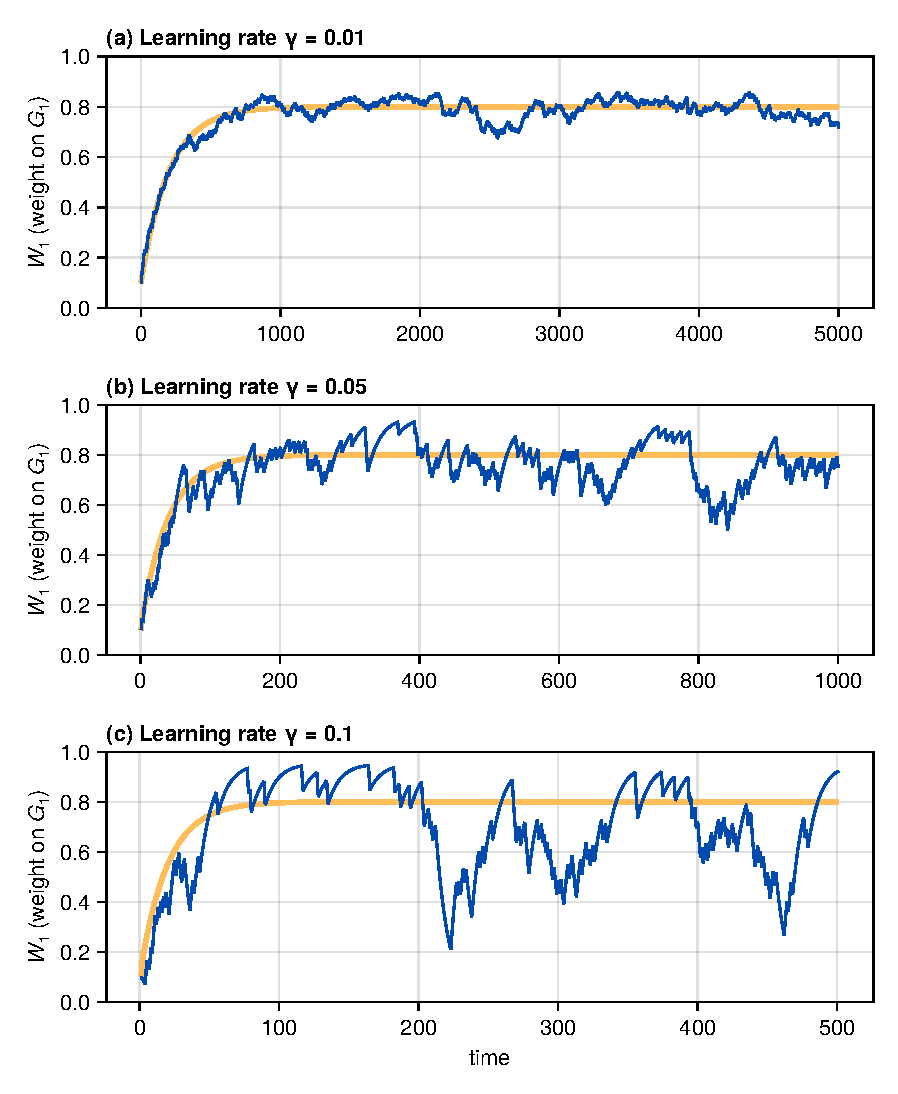
\includegraphics[width=1\textwidth]{figures/ch5/example-trajectories.pdf}
\caption{Three simulated learners, each in the same learning environment
characterized by penalty probabilities \(c_1 = 0.05\) and \(c_2 = 0.4\)
but with different learning rates: \(\gamma = 0.01\), \(\gamma = 0.05\)
and \(\gamma = 0.1\). Each learner additionally is subject to an
L2-difficulty of \(d = 0.05\). With these choices, the expected value of
\(W_1\) at stationarity is \(0.8\) (the thick yellow curve gives the
evolution of the expected value). With the parameters chosen, and with
each learner starting from \(W_1(0) = 0.1\), the stationary distribution
is reached after about the first \(10\gamma^{-1}\) learning iterations.
The weight \(W_2 = 1 - W_1\) is not shown.}\label{fig:trajectories}
}
\end{figure}

Since \(W_1 + W_2 = 1\), we may concentrate on \(W_1\), the weight on
the L2-difficult grammar \(G_1\), in what follows. The mean and variance
of \(W_1\) at stationarity may be expressed in closed form. Let
\(\textnormal{E}[W_1]\) stand for the mean (i.e.~expected value) and
\(\textnormal{Var}[W_1]\) for the variance of \(W_1\). It can be shown
that, at equilibrium, \begin{equation}
\textnormal{E}[W_1] = \frac{c_2}{c_1 + c_2 + d}
\label{eq:EP}\end{equation} and \begin{equation}
\textnormal{Var}[W_1] = 
- \textnormal{E}[W_1]^2
+ \frac{CG^2 + 2c_2 G \gamma}{1 - G^2 + 2 C G \gamma }  \textnormal{E}[W_1] 
+ \frac{c_2 \gamma^2}{1 - G^2 + 2 C G \gamma } 
\label{eq:VarP}\end{equation} with \(C = 1 - c_1 - c_2\) and
\(G = 1 - \gamma - \delta\) \autocite[see][Supplementary file, equations
(20) and (24)]{Kauhanen2022}.

A few remarks are in order. First, once statistical equilibrium has been
reached, the expected value of the learner's weight only depends on two
things: (i) the penalty probabilities \(c_1\) and \(c_2\), and (ii) the
L2-difficulty factor \(d\). In particular, this expected value is not
affected by the absolute magnitudes of the learning rate parameters. The
variance, on the other hand, is -- the higher the learning rates, the
higher the variance, and consequently the more fluctuations we observe
at equilibrium (Figure \ref{fig:trajectories}). This will play a crucial
role later when we break away from the deterministic limit.

Secondly, the expected weight on \(G_1\) (the grammar which contains the
L2-difficult feature) at equilibrium is always lower for an L2 learner
compared to an L1 learner, and the difference is greater the higher the
degree of L2-difficulty \(d\).

Thirdly, although we have not proved it here, the approach to
stationarity is exponential, meaning that the absolute difference
between the mean of the stationary distribution and the random
variable's current value decreases exponentially. This fact (which is
also apparent from the simulated trajectories in Figure
\ref{fig:trajectories}) is important for the following reason: we need
not in general worry about whether learners reach equilibrium;
convergence is quick. A related fact (again not strictly proven here) is
that the learner's initial state does not influence the stationary
distribution; the learner is ``ergodic'' and thus ultimately forgets
their initial state \autocite{NarendraThathachar1989}.

Most work on the variational learning model has assumed, for the sake of
tractability, that the variance does not exist at equilibrium
\autocites[e.g.][]{Yang2000,HeyWal2013,SimEtAl2019,Kauhanen2022}. This
allows one to assume that every learner in a population of learners is
described by a single number, namely the expectation
\(\textnormal{E}[W_1]\). It is then relatively straightforward to write
down an inter-generational equation (in either discrete or continuous
time) which describes how the weight in one generation of learners is
determined from the value of that weight in an immediately preceding
generation of learners (under the usual assumptions, this leads to a
sigmoidal ``S-curve'' at the population level; see
\cite{WallenbergEtAlDiaCom}). Section \ref{sec:bifurcation-threshold}
reviews this strategy particularly as it applies to the modelling of
contact-induced change. Section \ref{sec:embracing-variation}
reintroduces the variance; the remaining sections then ask to what
extent the predictions made by the deterministic limit continue to hold
when populations are not deterministic.

\hypertarget{sec:bifurcation-threshold}{%
\section{The deterministic limit and the bifurcation
threshold}\label{sec:bifurcation-threshold}}

In real populations, the penalty probabilities \(c_1\) and \(c_2\) of
the competing grammars may differ from learner to learner (depending on
which other language users they interact with) and need not remain
constant over the duration of learning. Analysing a model that attempts
to reproduce this reality incurs significant challenges -- the numerous
interdependencies between different language users in such a model mean
that analytical results are for all intents and purposes unobtainable.
It makes sense to start from a simpler vantage point, one which employs
a small set of simplifying assumptions that together render the model
analytically tractable. This is the approach adopted in
\textcite{Kauhanen2022}, briefly summarized next.

Assume a mixed population of L1 and L2 learners. Every learner
internalizes weights \(W_1\) and \(W_2\) for two grammars, as outlined
above. Let \(p\) refer to the probability of encountering an L1 learner
employing \(G_1\) at a given point in time (mathematically, this is
equivalent to the expected value of \(W_1\), aggregated over the L1
population). Similarly, let \(q\) refer to the probability of
encountering an L2 learner employing \(G_1\). The state of the
population is described by the pair of numbers \((p,q)\); since these
are probabilities, the state space is the unit square
\([0,1] \times [0,1]\). We now ask: what is the eventual fate of the
dynamics? Does the state \((p,q)\) tend to some definite value, and if
so, what is that value? Moreover, under what conditions do we have
\((p,q) \to (0,0)\), so that no one (the L1 learners included) uses the
L2-difficult grammar in the end?

Suppose the following assumptions are made:

\begin{enumerate}
\def\labelenumi{\arabic{enumi}.}
\tightlist
\item
  Learners are arranged in a discrete sequence of non-overlapping
  generations.
\item
  Each generation consists of infinitely many learners.
\item
  Each learner in generation \(n\) picks interlocutors from generation
  \(n-1\) uniformly at random.
\item
  There is zero variance at any learner's stationary distribution.
\end{enumerate}

\noindent Under these assumptions, \textcite{Kauhanen2022} shows that
\((p,q)\) tends to a global attractor \((p^*, q^*)\) which either is the
origin \((p^*, q^*) = (0,0)\) or lies in the interior of the unit
square. In the former case \(G_1\), the grammar with the responsive
feature, eventually gives way completely to grammar \(G_2\), which
incurs no L2-difficulty. It is important to note that, in this case, the
effects of L2-difficulty also percolate to the L1 learner population,
even though the latter themselves face no L2-difficulty in learning: the
presence of L2 learners shifts the linguistic input L1 learners are
exposed to, lowering the probability of them encountering strings which
are uniquely accepted by the L2-difficult grammar \(G_1\). Through this
mechanism, the effects of L2 learning may percolate through the whole
population -- at least in principle.

Whether this sort of ``total percolation'' or ``total simplification''
(total replacement of \(G_1\) by \(G_2\)) occurs depends on whether
\(\sigma\), the proportion of L2 learners in the population, exceeds a
critical threshold \(\sigma_\textnormal{crit}\) whose value is
\begin{equation}
\sigma_\textnormal{crit} = \bigg(1 - \frac{a_2}{a_1}\bigg)\bigg(1 + \frac{a_2}{d}\bigg)
\label{eq:bifurcation-threshold}\end{equation} \autocite[equation
19]{Kauhanen2022}. Note that the critical threshold is a relation
involving four parameters: the proportion of L2 learners (\(\sigma\)),
the amount of L2-difficulty experienced by the L2 learners (\(d\)), and
the advantages of the competing grammars (\(a_1\) and \(a_2\)).

Equation (\ref{eq:bifurcation-threshold}) can be used to make and test
predictions about the outcomes of individual language contact
situations. One of the empirical case studies considered in
\textcite{Kauhanen2022} concerns the expression of null subjects in
Afro-Peruvian Spanish (APS), a variety of Spanish spoken by descendants
of people brought as slaves to Colonial Peru in the 17th--19th
centuries. \textcite{SessaregoBook} argues that present-day APS exhibits
a mixed system of null subjects, analysable as grammar competition
between a consistent null subject grammar and a non-null subject
grammar. To illustrate, consider the use of overt subjects in
(\ref{ex:aps}), where Standard Peninsular Spanish would prescribe null
subjects.

\begin{exe}
\ex \label{ex:aps} 
\gll Paco fue a casa. Él se tomó una botella de cerveza y después él se fue al bar de fiesta. \\ 
Paco went to home he himself took a bottle of beer and afterwards he himself went {to the} bar of party \\
\trans `Paco went home. He drunk a bottle of beer and then went to the bar to have fun.' \hfill \parencite[382]{Ses2014}
\end{exe}

\noindent This proliferation of overt subjects is not unique to APS, but
rather has been documented in a number of varieties of Spanish which
historically were the objects of European colonialism (see Chapter
\ref{ch:gemma} for extended discussion and a typology of null subject
languages). Importantly, null subjects have been found to incur
L2-difficulty in a number of experimental studies
\autocite{Bini1993,PerGla1999,MargazaBel2006}, suggesting a plausible
psychosociolinguistic explanation for the move away from null subjects
in these languages. These remarks notwithstanding, APS did not lose null
subjects entirely, and (unlike for instance the genealogically closely
related French) is not classified as a non-null subject language today.
From the point of view of sociolinguistic typology, then, the challenge
in this particular empirical case study is to explain why, despite
obvious extensive linguistic admixture in Colonial Peru, APS did not
fully lose null subjects, but rather landed on a mixed system.

Using available demographic data (which is admittedly scant),
\textcite{Kauhanen2022} estimated the likely proportion of L2 learners
at around \(\sigma \approx 0.5\), while corpus estimates by
\textcite{SimEtAl2019} put the advantage of the null subject grammar
\(G_1\) at \(a_1 = 0.7\) and the advantage of the competing non-null
subject grammar \(G_2\) at \(a_2 = 0.05\). Although we at present lack
any empirical estimates of the magnitude of the L2-difficulty parameter
\(d\) in this (or indeed in any other) case, the critical value
\(\sigma_\textnormal{crit}\) has a lower bound which is attained as
\(d \to \infty\); this is \begin{equation}
\lim_{d \to \infty} \sigma_{\textnormal{crit}} = 1 - \frac{a_2}{a_1},
\label{eq:limit-of-sigma-crit}\end{equation} as is easy to verify from
(\ref{eq:bifurcation-threshold}). Plugging in the advantage parameters,
we find \begin{equation}
1 - \frac{a_2}{a_1} = 1 - \frac{0.05}{0.7} \approx 0.93.
\label{eq:aps-sigma-crit}\end{equation} Since obviously \(0.5 < 0.93\),
the prediction that APS settles on a mixed system is thus borne out. In
other words, in this case the great formal advantage (proportion of
input strings parsed) enjoyed by the null subject grammar in comparison
to the non-null subject grammar means that around 93\% of the population
would have had to be learning the language as an L2 for full
simplification to have taken place. The empirical value of the
proportion of L2 learners was almost certainly lower than this, and so
full simplification never took place.

Section \ref{sec:revisited} below will revisit the APS case study.
There, in the context of a full stochastic simulation of learning and
population dynamics, we will be in a position to examine exactly how far
from full simplification the language remained at the moment of greatest
influence from L2 learning.

\hypertarget{sec:embracing-variation}{%
\section{Embracing variation}\label{sec:embracing-variation}}

Adopting the simplifying assumptions listed in the previous section made
it possible to derive equation (\ref{eq:bifurcation-threshold}), the
bifurcation threshold for contact-induced simplification in the
deterministic limit. In relation to real-world application, this result
suffers from the following main limitations, which arise immediately
from the simplifying assumptions made:

\begin{enumerate}
\def\labelenumi{\arabic{enumi}.}
\tightlist
\item
  It assumes \emph{complete and random mixing}. Everybody can come into
  contact with everybody else; in particular, there is no sense in which
  L2 learners might be more likely to interact among each other than
  with L1 learners (as might have been realistically the case in, for
  instance, the sorts of colonial settings which gave rise to languages
  such as APS).
\item
  It does not allow for \emph{variation between learners in the same
  (L1/L2) group}. Yet the L2 acquisition literature abounds in empirical
  data which strongly suggests that some individuals attain higher
  fluency than others, and even the usage patterns of L1 speakers vary
  from person to person.
\item
  It assumes a \emph{constant proportion of L2 learners \(\sigma\)}.
  However, in several empirically interesting situations (including the
  history of APS), it is the case that \(\sigma\) first goes up, then
  comes down again as the children of immigrants acquire the language as
  an L1 rather than as an L2.
\end{enumerate}

Relaxing these assumptions requires us to view the system as an
agent-based model \autocite{Gilbert2020,Smaldino2023} and to run
computer simulations, something that introduces a number of technical
challenges. For instance, even though it was pointed out above that the
approach to a learner's stationary distribution is exponential, this may
still take thousands of learning iterations depending on the specific
values of the learning rate parameters and the penalty probabilities. If
there are thousands of learners in the population, the numbers quickly
multiply, leading to long simulation runtimes. While this is often not a
problem from the point of view of running a single simulation, a single
simulation outcome is never sufficient to give anything approaching a
complete picture of the model's possible behaviours. First, to
understand the role played by stochastic factors, the outcomes of
multiple simulation runs must be summarized (typically by taking
averages). Secondly, and more importantly, the many model parameters
involved result in a combinatorial explosion if we wish to sweep over
the parameter space in systematic fashion.

To illustrate this, suppose it took one minute to run a single
simulation of interest -- a reasonable estimate for a reasonably complex
model run on a modern computer. If there are three model parameters,
each of which can take on 10 different values, then running the
simulation for all possible model parameter combinations will take
\(10^3\), i.e.~one thousand, minutes. This corresponds to about 16
hours, still a reasonable time to wait perhaps. But now note that, as
emphasized above, we may wish to repeat the simulation for each model
parameter combination a number of times, say 50 times, to be able to
assess the effect of stochastic factors. Unless it is possible to
parallelize the simulation code, this immediately raises the runtime to
830 hours, or just over one month. Adding just one more model parameter
to the sweep (assuming again 10 different possible values for the
parameter) multiplies the runtime by 10, requiring us to wait 10 months
for our results. Requiring more resolution of the parameter sweep
(e.g.~100 possible values for each parameter) is clearly impossible in
practice, unless we have access to a supercomputer.

It is here that the availability of some analytical results becomes very
useful. As explained in Section \ref{sec:responsive-features}, in a
stationary learning environment the behaviour of learners may be
summarized by the properties of the distribution of \(W_1\) at
statistical equilibrium. Although the exact distribution is unknown, its
mean and variance can be computed. It turns out that these are enough to
characterize that distribution in practice.

Specifically, we adopt the following strategy -- which could be termed
the ``Beta approximation'' -- in the following simulations.\footnote{The
  Beta distribution is a continuous probability distribution over the
  interval \([0, 1]\) and is thus a suitable choice for describing the
  distribution of a random variable such as our \(W_1\). It is
  parameterized by two parameters, \(\alpha > 0\) and \(\beta > 0\),
  which determine the distribution's shape \autocite[see
  e.g.][151--152]{Samaniego2014}. For a different kind of application of
  a Beta approximation in linguistics (in the context of a
  Wright--Fisher model of language change), see
  \textcite{GuerreroEtAl2025}.} Instead of simulating each learner's
learning trajectory up to statistical equilibrium, we sample the
learner's ultimate value of \(W_1\) from a Beta distribution with
suitable shape parameters \(\alpha\) and \(\beta\). The shape parameters
are obtained via moment matching, as explained next. The mean and
variance of the Beta distribution are \begin{equation}\label{eq:mu}
\mu = \frac{\alpha}{\alpha + \beta}
\end{equation} and \begin{equation}\label{eq:sigma}
\sigma^2 = \frac{\alpha\beta}{(\alpha + \beta)^2(\alpha + \beta + 1)}
\end{equation} respectively \autocite[see e.g.][151]{Samaniego2014}.
Thus, to obtain a Beta distribution with a desired mean and variance, we
simply need to solve the above equations for the shape parameters
\(\alpha\) and \(\beta\), and plug in the mean and variance. But since
we know the mean and variance of the learner's stationary distribution,
we may now use these numbers to obtain a Beta distribution that
approximates that stationary distribution.

To illustrate, Figure \ref{fig:experiment} shows the results of a number
of experiments; model parameters were drawn at random and are listed in
Table \ref{tbl:experiment}. In each experiment, 10,000 learners were
simulated up to statistical equilibrium. The histograms depict that
equilibrium, i.e.~the distribution of \(W_1\) across all 10,000 learners
at equilibrium.\footnote{In fact, since the learning scheme is ergodic
  and each learner within a given experiment faces the same learning
  environment (the same penalty probabilities \(c_1\) and \(c_2\)) and
  employs the same learning rate parameters, the same result could be
  obtained by sampling 10,000 values from the stationary distribution of
  a single learner.} The curves give the probability density of the Beta
distribution found through the method of moment matching. It is evident
that, in each case (i.e.~for different values of the model parameters
\(c_1\), \(c_2\), \(\gamma\) and \(\delta\)), the agreement is very
good, justifying the use of the Beta approximation.

\begin{figure}
\hypertarget{fig:experiment}{%
\centering
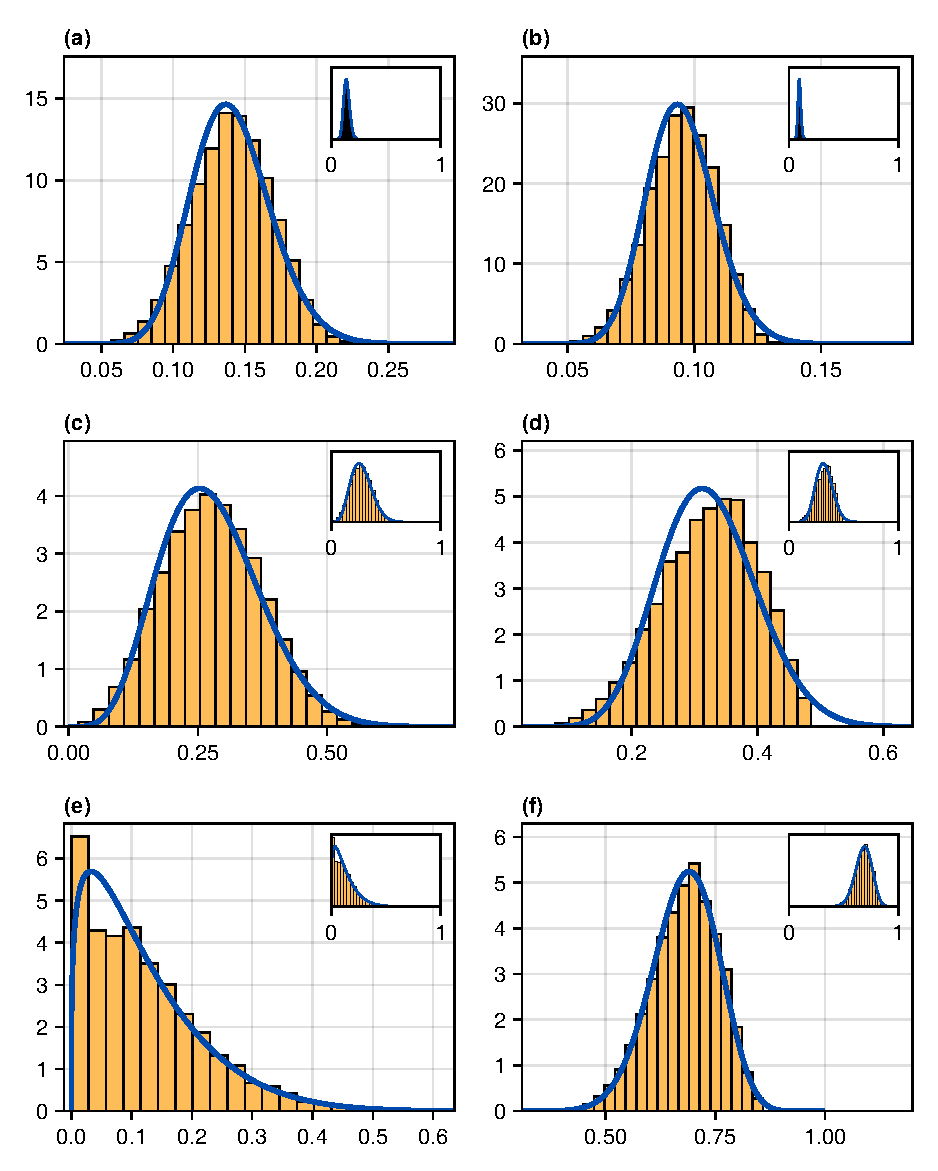
\includegraphics[width=1\textwidth]{figures/ch5/experiment.pdf}
\caption{Six learning simulation experiments. In each experiment, 10,000
learners were simulated to equilibrium with randomly drawn parameters
(see Table \ref{tbl:experiment}). The equilibrium distribution of
\(W_1\), the weight on \(G_1\) (yellow histogram), is well approximated
by a Beta distribution (blue curves indicating the probability density
function) found by moment matching. Insets scale each facet to the
entire range of possible values of \(W_1\), the interval
\([0,1]\).}\label{fig:experiment}
}
\end{figure}

\begin{table}
\caption{Model parameters ($c_1$, $c_2$, $\gamma$ and $\delta$; randomly drawn) for the simulation experiments of Figure \ref{fig:experiment}, together with the mean ($\E[W_1]$) and variance ($\textnormal{Var}[W_1]$) of the stationary distribution (\ref{eq:mu}--\ref{eq:sigma}) and the moment-matched shape parameters ($\alpha$, $\beta$) of the approximating Beta distribution.}\label{tbl:experiment}
\begin{tabular}{lrrrrrrrr}
\toprule
 & $c_1$ & $c_2$ & $\gamma$ & $\delta$ & $\textnormal{E}[W_1]$ & $\textnormal{Var}[W_1]$ & $\alpha$ & $\beta$ \\
\midrule
(a) & 0.94 & 0.66 & 0.027 & 0.083 & 0.14 & 0.0008 & 22.6 & 137.6 \\
(b) & 0.87 & 0.73 & 0.012 & 0.073 & 0.1 & 0.0002 & 45.3 & 431.1 \\
(c) & 0.34 & 0.31 & 0.081 & 0.038 & 0.28 & 0.0091 & 5.8 & 15.2 \\
(d) & 0.14 & 0.57 & 0.085 & 0.09 & 0.32 & 0.0058 & 11.8 & 24.9 \\
(e) & 0.32 & 0.09 & 0.1 & 0.033 & 0.12 & 0.0093 & 1.3 & 9.2 \\
(f) & 0.25 & 0.87 & 0.082 & 0.013 & 0.68 & 0.0056 & 25.5 & 12.0 \\
\bottomrule
\end{tabular}
\end{table}

As a consequence, simulation runtimes are drastically reduced. On the
computer used to simulate the above experiments,\footnote{A PC with an
  Intel Core i5-13600KF processor and 128 GB of DDR4 RAM. All simulation
  code was written in Julia \autocite{Julia}, version 1.11.4, and can be
  obtained from
  \url{https://github.com/erc-starfish/contact-simulations}.} the mean
runtime for simulating one learner to equilibrium was on the order of
three hundred microseconds. By contrast, sampling from the Beta
distribution only took around one hundred and fifty nanoseconds on
average, meaning that the latter operation is a couple thousand times
(more than three orders of magnitude) faster.

\hypertarget{sec:simulation-setup}{%
\section{Simulation setup}\label{sec:simulation-setup}}

For the agent-based simulations, the following setup is assumed.
Simulations are carried out on a spatial substrate which is a regular
two-dimensional lattice of \(L_h \times L_v\) sites with
non-periodic\footnote{This means that the lattice does not ``wrap
  around'' at its edges.} boundaries, \(L_h\) giving the lattice side
length in the horizontal dimension and \(L_v\) that in the vertical
dimension. While L1 learning may occur in any part of this space, L2
learning is constrained to occur only in the lower half of the lattice
(i.e.~in sites with a vertical index less than half of \(L_v\)). The
shape of the lattice is varied through the use of an \emph{aspect ratio}
parameter \(\rho\), defined as the ratio of lattice width to lattice
height. For \(\rho > 1\), the lattice is wider than it is tall, and for
\(\rho < 1\), it is taller than it is wide (see Figure
\ref{fig:rho}).\footnote{Concretely, the horizontal and vertical
  dimensions are set as \(L_h = \lfloor \sqrt{\rho L} \rfloor\) and
  \(L_v = \lfloor \sqrt{\rho^{-1} L} \rfloor\) where \(L\) is the
  approximate desired total number of sites on the lattice.}

\begin{figure}
\hypertarget{fig:rho}{%
\centering
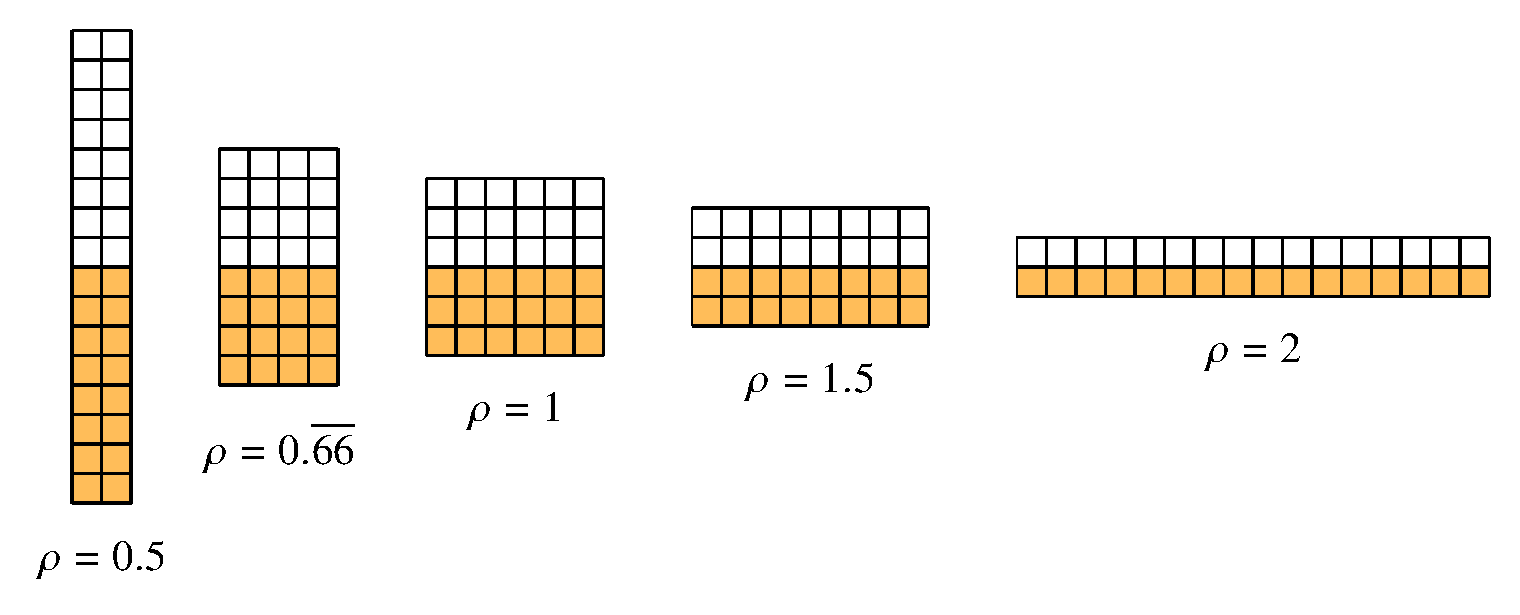
\includegraphics[width=0.95\textwidth]{figures/ch5/lattice.pdf}
\caption{The aspect ratio parameter \(\rho\) is used to set the relative
horizontal and vertical dimensions of the lattice. L2 learning is
constrained to occur only in the bottom half of the lattice (yellow),
and so \(\rho\) implicitly controls the length of the interface between
the initial L1 and L2 learning regions. (Lattices in the actual
simulations are far larger, with a total of \(L \approx 5000\)
sites.)}\label{fig:rho}
}
\end{figure}

The decision to constrain L2 learning to the lower half of the lattice,
and the use of the aspect ratio parameter \(\rho\), together allow us to
control the intensity of the initial interactions between L1 and L2
learners, i.e.~interactions between the top and bottom halves of the
lattice. This structure may be interpreted either as spatial (as in many
situations of language contact between two contiguous geographical
regions) or as social (as in situations of colonization and slavery) in
origin. In a very rudimentary way, this will allow us to probe different
kinds of scenarios of language contact \autocite[cf.][]{Muysken2013}.

Simulations proceed in discrete time, each time step interpreted as one
year of real time. At each time step, three actions are performed:

\paragraph*{1. Birth and L1 acquisition.}

A number of speakers are created and made to undergo the process of L1
acquisition. The number of speakers ``born'' this way is proportional to
(i) a birth rate parameter, \(b\), (ii) the current population size,
\(N\), and (iii) a carrying capacity, \(K\); the latter ensures that
population sizes do not explode exponentially (which would lead to
computationally intractable, and also empirically unrealistic,
simulation runs).\footnote{For a listing of all model parameters along
  with their default values, see Table \ref{tbl:parameters}.}
Concretely, the number of newborn speakers is sampled from a binomial
distribution with success probability \(b\) and number of trials
\(\lfloor N(1 - (N/K)) \rfloor^+\), where
\(\lfloor x \rfloor^+ = \lfloor x \rfloor\) (i.e.~the integer part of
\(x\)) if \(x \geq 0\) and \(\lfloor x \rfloor^+ = 0\) if \(x < 0\).
Each newborn speaker is assigned to a lattice site at most \(R\) sites
away from the site occupied by a randomly chosen already existing
speaker, the latter interpreted as the newborn's parent. Multiple
speakers may occupy the same site; once placed on the lattice, a speaker
stays in the same site for its lifetime. L1 acquisition is modelled by
sampling from a Beta distribution as explained in Section
\ref{sec:embracing-variation}. The learner estimates the penalty
probabilities \(c_1\) and \(c_2\) from its local environment.
Concretely, the learner samples \(F\) speakers at random from within a
distance (Chebyshev distance) of \(R\) on the lattice, or takes all
neighbouring speakers if their number does not exceed \(F\). The local
penalty probabilities \(c_1\) and \(c_2\) are then calculated from the
frequencies of use of grammars \(G_1\) and \(G_2\) among these
neighbours, together with the advantage parameters \(a_1\) and \(a_2\),
in the usual manner: if \(x\) stands for the local frequency of \(G_1\),
then \(c_1 = a_2(1-x)\) and \(c_2 = a_1x\)
\autocite{Yang2000,WallenbergEtAlDiaCom}.

\paragraph*{2. Immigration and L2 acquisition.}

A number of speakers are ``imported'' into the lattice and made to
undergo the process of L2 acquisition. The number of immigrants is, like
the number of newborn agents in step 1, dependent on both the current
population size and the carrying capacity, and is similarly sampled from
a binomial distribution, except that a migration rate parameter \(m\) is
used instead of the birth rate \(b\). This way of arranging the
immigration process is modelled on the assumptions that (i) larger
populations attract more immigration, and (ii) a finite substrate can
support only a finite amount of immigration. L2 acquisition proceeds as
L1 acquisition, via the Beta approximation, except that the learner is
also subject to the L2-difficulty parameter \(d\), set as a global
parameter for all learners.

In Appendix A, it is shown that given the above general assumptions
about population dynamics, the expected proportion of L2 learners in the
population is \begin{equation}
\textnormal{E}[\sigma] = \frac{m}{b + m}
\label{eq:E-sigma}\end{equation} once the total population size has
stabilized. In other words, this quantity may readily be computed from
the birth and immigration rates \(b\) and \(m\). Conversely, in order to
obtain a desired expected proportion of L2 speakers
\(\textnormal{E}[\sigma]\) having set some fixed birth rate \(b\), we
may invert the above equation to verify that the immigration rate \(m\)
needs to be chosen so that \begin{equation}
m = \frac{\textnormal{E}[\sigma]}{1 - \textnormal{E}[\sigma]} b.
\label{eq:tau}\end{equation} In the following simulations, this is what
we do: i.e.~rather than directly set the immigration rate \(m\), we set
the desired proportion of L2 learners \(\E[\sigma]\) and calculate \(m\)
using (\ref{eq:tau}).

\paragraph*{3. Death.}

When agents are introduced to the population, they are assigned an age
which is 0 for L1 learners and a random number for L2 learners; this
random number is constructed by drawing a number from a Gamma
distribution with shape parameter \(\phi\) and scale parameter
\(\theta\). Agents are also assigned a lifetime, sampled from a Weibull
distribution\footnote{The Weibull distribution is a standard choice for
  modelling the probability of time-until-failure, whether in engineered
  or biological systems \autocite[see][155--156]{Samaniego2014}.} with
shape parameter \(k\) and scale parameter \(\lambda\). At each
simulation iteration, the age of every agent on the lattice is
incremented by one, and agents whose ages exceed their lifetimes are
removed from the lattice. The particular choices of \(k\) and
\(\lambda\) used in the simulations (see Table \ref{tbl:parameters})
imply that the survival distribution is left-skewed, meaning that death
is more likely the older a speaker becomes.

Figure \ref{fig:distros} provides example illustrations of the
distributions governing the above-described dynamics.

\begin{table}\caption{Overview of model parameters for the agent-based simulations in Sections \ref{sec:simulation-setup}--\ref{sec:sweeps}. Parameters which are held constant across all simulations reported in this and the following section are indicated with those constant values. Parameters with values labelled `various' were varied across simulations, as explained in more detail below.}\label{tbl:parameters}\begin{tabular}{lcr}
\toprule
Parameter & Symbol & Value(s) \\
\midrule
Advantage of grammar $G_1$ & $a_1$ & various \\
Advantage of grammar $G_2$ & $a_2$ & various \\
Learning rate & $\gamma$ & various \\
L2-difficulty of $G_1$ & $d$ & various \\
Lattice aspect ratio & $\rho$ & various \\
Approximate lattice size (number of sites) & $L$ & 5000 \\
Interaction radius & $R$ & 10 \\
Maximum interaction density (number of contacts) & $F$ & 50 \\
Birth rate & $b$ & 0.05 \\
Expected proportion of L2 learners & $\textnormal{E}[\sigma]$ & various \\
Length of immigration period & $T_\textnormal{L2}$ & various \\
Shape of immigration age distribution & $\phi$ & 6.0 \\
Scale of immigration age distribution & $\theta$ & 5.0 \\
Number of L1 speakers at time 0 & $N_0$ & 100 \\
Shape parameter of death distribution & $k$ & 10.0 \\
Scale parameter of death distribution & $\lambda$ & 70.0 \\
Population carrying capacity & $K$ & various \\
Length of simulation & $T$ & various \\
\bottomrule
\end{tabular}
\end{table}

\begin{figure}
\hypertarget{fig:distros}{%
\centering
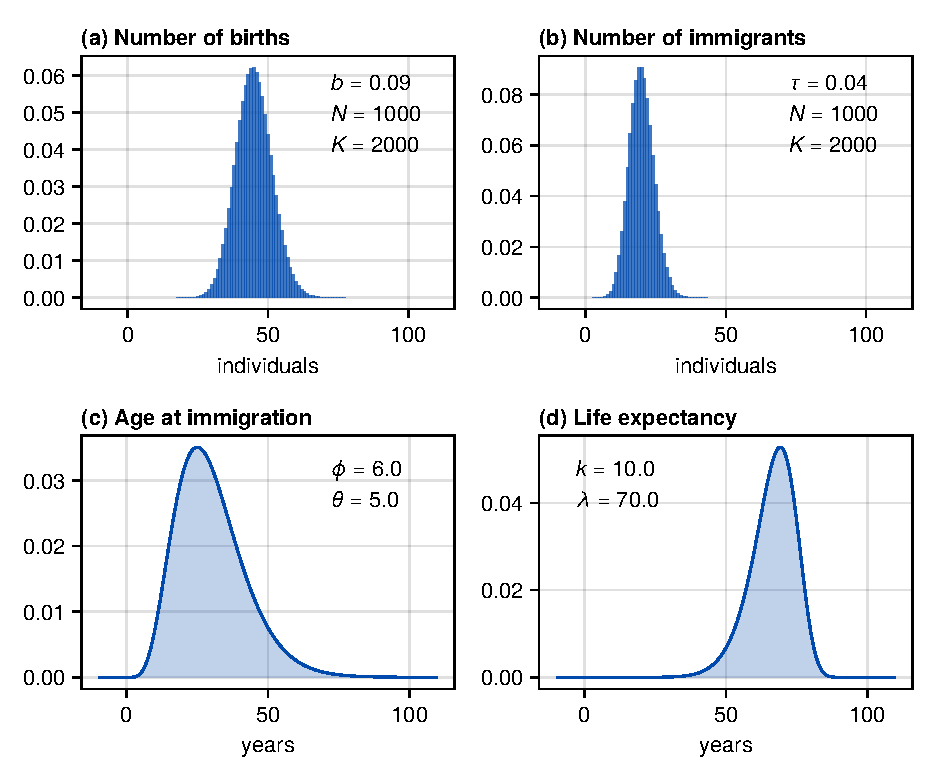
\includegraphics[width=1\textwidth]{figures/ch5/distros.pdf}
\caption{Probability mass (a--b) or density (c--d) functions of example
distributions for (a) number of births per year, (b) number of
immigrants per year, (c) age of immigrants, and (d) life expectancy of
individuals, given the parameters in the plot
insets.}\label{fig:distros}
}
\end{figure}

Each simulation is initialized with 100 L1 speakers with full use of
\(G_1\) (\(W_1 = 1\)) inserted in random locations of the L1 portion of
the lattice. From here, the simulation proceeds according to the above
description, with the exception that for the first 50 years, there is no
immigration. This is to ascertain that full use of \(G_1\) is in fact a
stable population equilibrium in the absence of L2 learning. After the
first 50 years, immigration is enabled and continues for the following
\(T_\textnormal{L2}\) years. This parameter allows us to control the
temporal extent of the immigration process, facilitating the modelling
of both situations of temporally extended moderate bilingualism and more
radical population dynamics such as those of colonial societies, which
are characterized by strong initial immigration followed by its
levelling off at abolition. Each simulation is run for a total of \(T\)
time steps. The main observable of interest is the population average of
\(W_1\), i.e.~the mean usage of the L2-difficult grammar \(G_1\),
throughout and, in particular, at the end of the simulation.

It is important to emphasize that while L2 acquisition is constrained to
only occur in the lower half of the lattice, no such constraint is in
place for L1 acquisition. Thus, when L2 learners have children
(i.e.~when newborn speakers are placed in the vicinity of existing
speakers in the lower half of the lattice), those children undergo their
acquisition process as L1 learners.

Figure \ref{fig:ts} illustrates a typical simulation run, plotting the
mean weight on \(G_1\), the proportion of L2 learners, and normalized
population size (the number of speakers divided by its maximum value
over the duration of the simulation) against time, for the simulation
parameters listed in Table \ref{tbl:onerun}. As L2 learners are
introduced into the population from time 50 onwards, we observe a steady
decrease in the mean weight on \(G_1\). Concomitantly, the proportion of
L2 learners increases with the influx of these learners. Ultimately, the
weight on \(G_1\) tends toward zero; this aligns with the prediction of
the deterministic model, as the proportion of L2 learners exceeds the
critical threshold \(\sigma_\textnormal{crit}\) given the parameter
values of Table \ref{tbl:onerun}. The L2-difficult grammar is not
recovered, at least not instantly, even when the supply of L2 learners
is cut off later.

\begin{table}\caption{Model parameters for the simulation depicted in Figures \ref{fig:ts}--\ref{fig:lat}. For the values of the constant parameters, consult Table \ref{tbl:parameters}.}\label{tbl:onerun}\begin{tabular}{lcr}
\toprule
Parameter & Symbol & Value(s) \\
\midrule
Advantage of grammar $G_1$ & $a_1$ & 0.12 \\
Advantage of grammar $G_2$ & $a_2$ & 0.1 \\
Learning rate & $\gamma$ & 0.01 \\
L2-difficulty of $G_1$ & $d$ & 10 \\
Lattice aspect ratio & $\rho$ & 1.5 \\
Expected proportion of L2 learners & $\textnormal{E}[\sigma]$ & 0.7 \\
Length of immigration period & $T_\textnormal{L2}$ & 200 \\
Population carrying capacity & $K$ & 20000 \\
Length of simulation & $T$ & 500 \\
\bottomrule
\end{tabular}
\end{table}

Figure \ref{fig:lat} provides an alternative view of the same simulation
run. Each of the six panels of this figure provides a snapshot of the
lattice at a different point in time, with crosses indicating speakers
(upright crosses \(=\) L1 learners, slanted crosses \(=\) L2 learners;
red \(=\) higher weight on \(G_1\), blue \(=\) lower weight on \(G_1\)).
To promote legibility, a random sample of 1\% of all speakers is drawn,
and at slightly jittered locations.

\begin{figure}
\hypertarget{fig:ts}{%
\centering
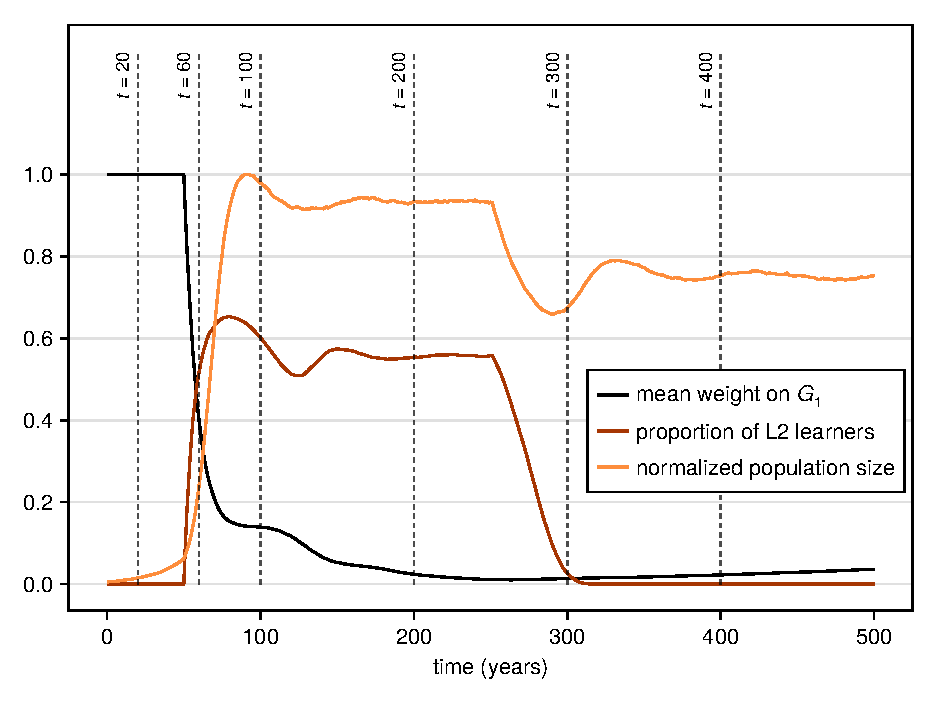
\includegraphics[width=1\textwidth]{figures/ch5/ts.pdf}
\caption{One simulation run. For model parameters, see Table
\ref{tbl:onerun}. Snapshots of the population at the indicated time
points are provided in Figure \ref{fig:lat}.}\label{fig:ts}
}
\end{figure}

\begin{figure}
\hypertarget{fig:lat}{%
\centering
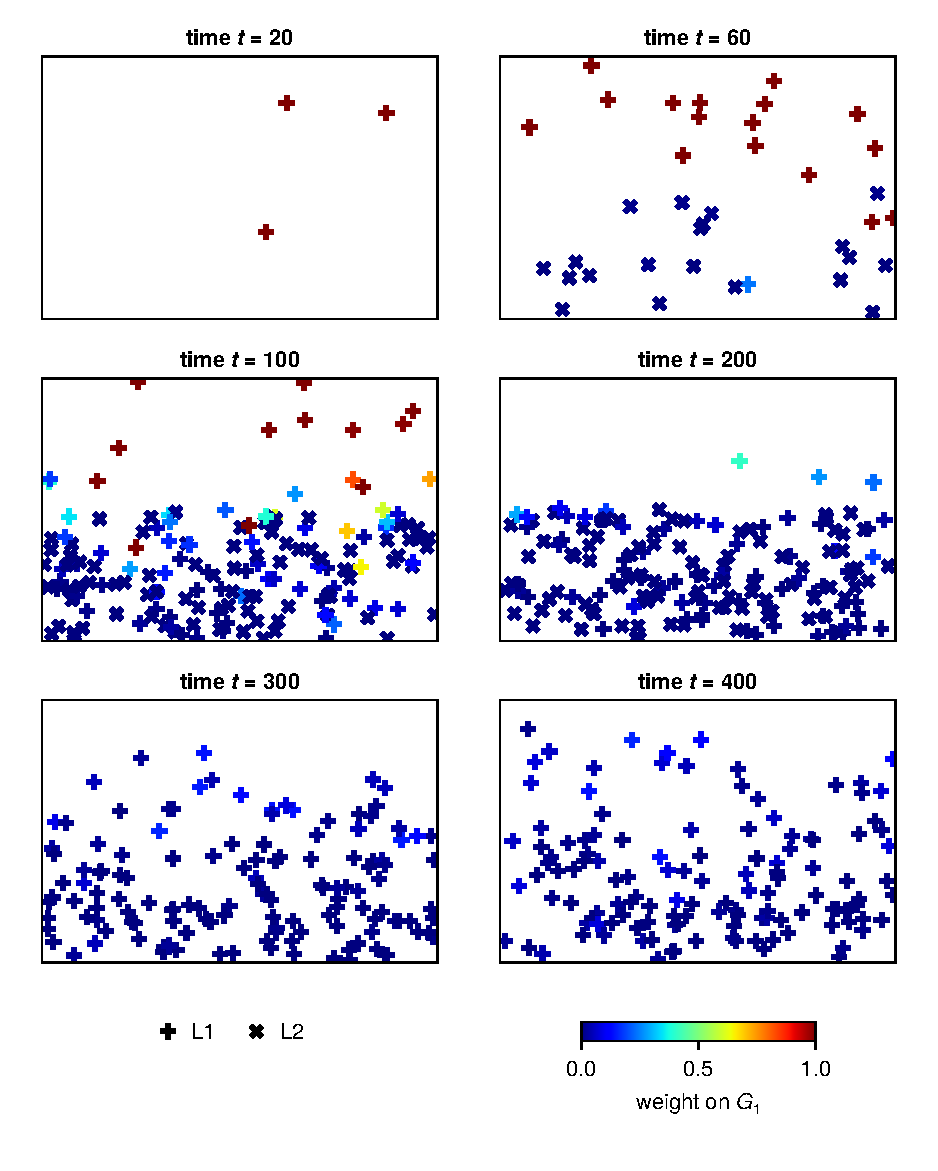
\includegraphics[width=1\textwidth]{figures/ch5/lat.pdf}
\caption{Snapshots from a simulation with the parameters of Table
\ref{tbl:onerun}. Each cross represents one speaker in its position on
the lattice (a random sample of 1\% of all speakers is actually
visualized, and speaker positions are slightly jittered, for reasons of
legibility). Upright crosses represent L1 learners, slanted crosses L2
learners. Colour corresponds to the speaker's weight on the L2-difficult
grammar \(G_1\).}\label{fig:lat}
}
\end{figure}

\hypertarget{sec:sweeps}{%
\section{Systematic parameter sweeps}\label{sec:sweeps}}

In all, the simulation setup described in the previous section involves
18 model parameters. If one were to carry out a systematic parameter
sweep across this parameter space with, say, 10 values per parameter and
50 repetitions for each parameter combination, the number of simulation
runs would equal \(50 \times 10^{18}\). This is intractable even with
the Beta approximation. Some insight is thus required in identifying
what parameters are likely to be of interest. This, in turn, requires us
to formulate specific research questions.

In what follows, I will focus on the following two questions:

\begin{enumerate}
\def\labelenumi{\arabic{enumi}.}
\tightlist
\item
  Does the bifurcation threshold identified in the deterministic limit
  (\ref{eq:bifurcation-threshold}) retain its validity in this
  stochastic simulation setup?
\item
  How do language contact outcomes depend on (i) interaction patterns
  between the subpopulations (i.e.~on lattice aspect ratio \(\rho\)) and
  (ii) the length of the period of language contact (i.e.~the length of
  immigration parameter \(T_\textnormal{L2}\))?
\end{enumerate}

To probe question 1, a sweep was carried out by varying the parameters
\(\textnormal{E}[\sigma]\), the expected proportion of L2 learners, and
\(d\), the extent of L2-difficulty on grammar \(G_1\) (see Table
\ref{tbl:bifu} for model parameters). For each combination of
\(\textnormal{E}[\sigma]\) and \(d\), 50 simulations were carried out,
each simulation lasting 3000 time steps (i.e.~3000 years of real time).
As explained above, L2 learning was enabled from time step 50; moreover,
in this particular sweep, the supply of L2 learners was never cut off.

For each combination of proportion of L2 learners \(\sigma\) and
L2-difficulty \(d\) (and advantage parameters \(a_1\) and \(a_2\); see
Table \ref{tbl:bifu}), equation (\ref{eq:bifurcation-threshold})
predicts a specific threshold \(\sigma_\textnormal{crit}\). This
threshold is depicted in Figure \ref{fig:bifu} as the thick dashed line.
The heatmap provides the eventual value of \(W_1\) (weight on \(G_1\)),
averaged over the population and over all 50 simulation runs.
Furthermore, contour lines are drawn for \(W_1\) across this heatmap. We
find that the stochastic simulations are in general agreement with the
theoretical (deterministic-limit) prediction, with the following
difference: the theoretical calculation appears to somewhat overestimate
the extent of simplification. In other words, the contour line closest
to the theoretically predicted \(\sigma_\textnormal{crit}\) is 0.01,
corresponding to 1\% use of \(G_1\) across the entire population. This
is likely due to the presence of local influences in the stochastic
model: in contrast to the deterministic-limit prediction, which assumes
that every speaker comes in contact with every other speaker equally
frequently, in the stochastic simulation here variants may survive in
local ``pockets'' for considerable lengths of time.

\begin{figure}
\hypertarget{fig:bifu}{%
\centering
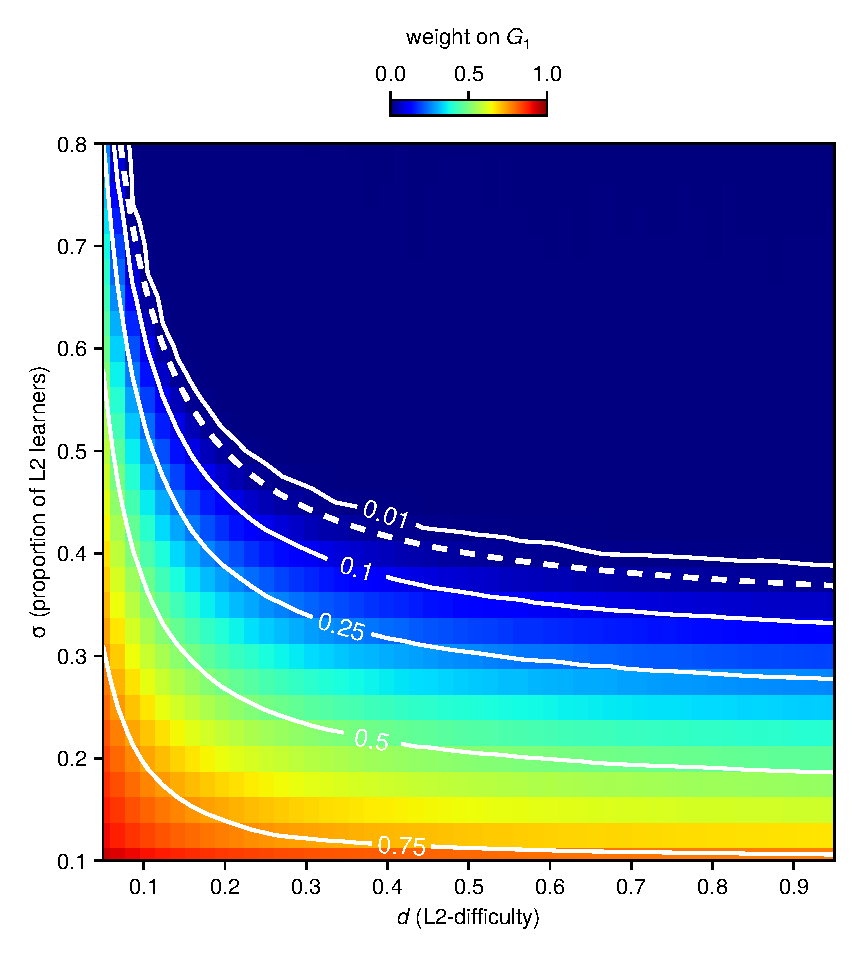
\includegraphics[width=1\textwidth]{figures/ch5/bifu.pdf}
\caption{Weight on the L2-difficult grammar \(G_1\) in the long run, as
a function of various choices of L2-difficulty \(d\) and proportion of
L2 learners \(\sigma\) (actual, not expected, proportion recorded at the
end of simulation). The thick dashed curve gives the critical threshold
(\ref{eq:bifurcation-threshold}) predicted by the deterministic model.
Solid curves are contour lines. For simulation parameters, see Table
\ref{tbl:bifu}.}\label{fig:bifu}
}
\end{figure}

Turning to question 2, a second sweep was performed for varying lattice
aspect ratios \(\rho\) and varying durations of the L2 learning period
\(T_\textnormal{L2}\) (for all model parameters, see Table
\ref{tbl:latshape}). Again, 50 simulations were carried out for every
simulation combination, for 3000 time steps. Figure \ref{fig:latshape}
visualizes the results, with time step on the horizontal axis, aspect
ratio \(\rho\) on the vertical axis, and \(T_\textnormal{L2}\) varying
across the panels. We observe an interaction between \(\rho\) and
\(T_\textnormal{L2}\) -- for short periods \(T_\textnormal{L2}\), tall
lattices (\(\rho < 1\)) conserve the simplification longer than do wide
lattices (\(\rho > 1\)). With higher \(T_\textnormal{L2}\), the effect
effectively disappears.

\begin{table}\caption{Model parameters for the sweep of Figure \ref{fig:bifu}. For the values of the constant parameters, consult Table \ref{tbl:parameters}. In this and subsequent tables, the notation $[a \stackrel{n}{\dots} b]$ refers to a sequence of $n$ equally-spaced values from $a$ to $b$ (endpoints inclusive). The notation $\log_{10}[a \stackrel{n}{\dots} b]$ refers to such a sequence with logarithmic spacing.}\label{tbl:bifu}\begin{tabular}{lcr}
\toprule
Parameter & Symbol & Value(s) \\
\midrule
Advantage of grammar $G_1$ & $a_1$ & 0.15 \\
Advantage of grammar $G_2$ & $a_2$ & 0.1 \\
Learning rate & $\gamma$ & 0.01 \\
L2-difficulty of $G_1$ & $d$ & [0.05 $\stackrel{50}{\ldots}$ 0.95] \\
Lattice aspect ratio & $\rho$ & 1.0 \\
Expected proportion of L2 learners & $\textnormal{E}[\sigma]$ & [0.1 $\stackrel{500}{\ldots}$ 0.9] \\
Length of immigration period & $T_\textnormal{L2}$ & 2950 \\
Population carrying capacity & $K$ & 1000 \\
Length of simulation & $T$ & 3000 \\
\bottomrule
\end{tabular}
\end{table}

\begin{table}\caption{Model parameters for the sweep of Figure \ref{fig:latshape}. For the values of the constant parameters, consult Table \ref{tbl:parameters}.}\label{tbl:latshape}\begin{tabular}{lcr}
\toprule
Parameter & Symbol & Value(s) \\
\midrule
Advantage of grammar $G_1$ & $a_1$ & 0.12 \\
Advantage of grammar $G_2$ & $a_2$ & 0.1 \\
Learning rate & $\gamma$ & 0.01 \\
L2-difficulty of $G_1$ & $d$ & 10 \\
Lattice aspect ratio & $\rho$ & $\log_{10}$[0.001 $\stackrel{50}{\ldots}$ 1000.0] \\
Expected proportion of L2 learners & $\textnormal{E}[\sigma]$ & 0.7 \\
Length of immigration period & $T_\textnormal{L2}$ & [100 $\stackrel{6}{\ldots}$ 600] \\
Population carrying capacity & $K$ & 10000 \\
Length of simulation & $T$ & 3000 \\
\bottomrule
\end{tabular}
\end{table}

\begin{figure}
\hypertarget{fig:latshape}{%
\centering
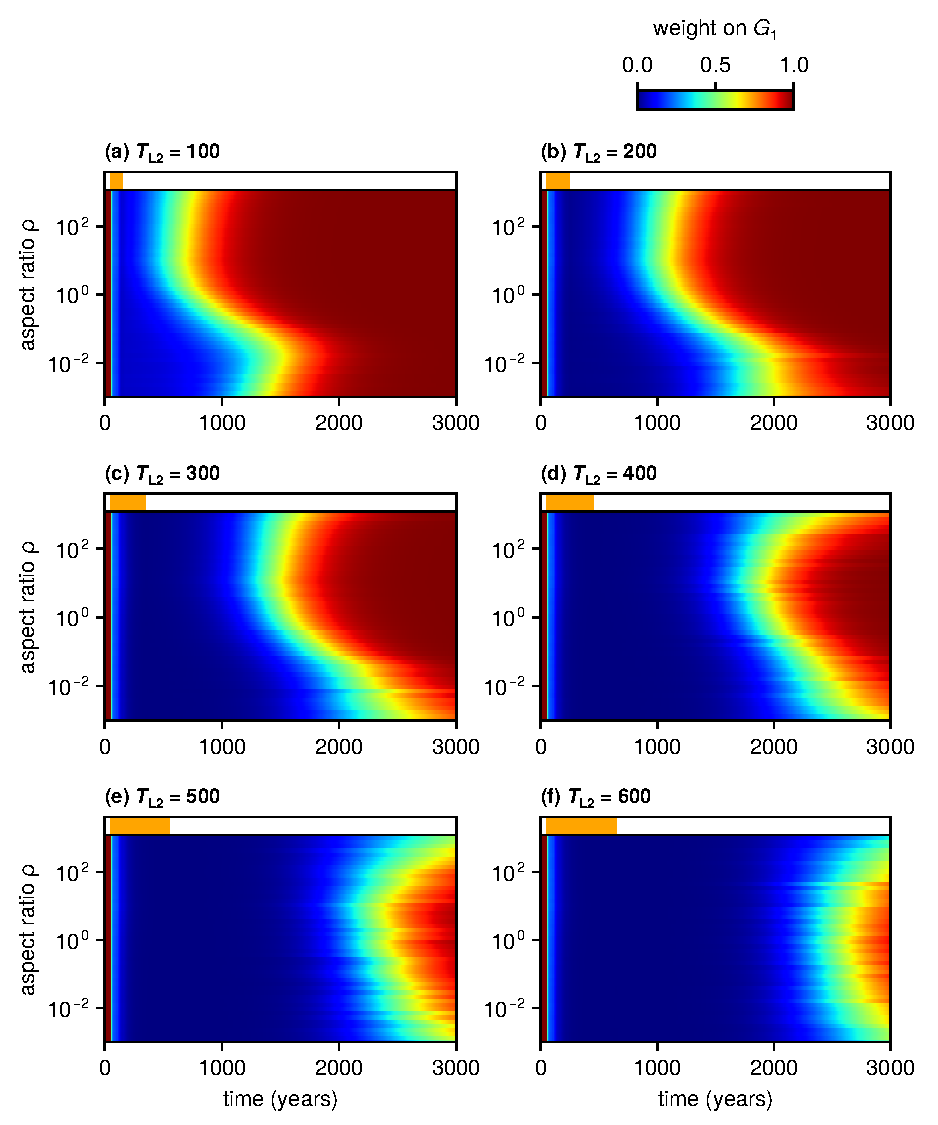
\includegraphics[width=1\textwidth]{figures/ch5/latshape.pdf}
\caption{Results of a parameter sweep crossing lattice aspect ratio
(\(\rho\)) and the length of the period of L2 learning/immigration
(\(T_\textnormal{L2}\)). The horizontal axis in each facet represents
simulation time step; the period of L2 learning is depicted by the
orange bar at the top of each panel.}\label{fig:latshape}
}
\end{figure}

This interaction with short periods of L2 learning may seem
counterintuitive at first: wide lattices (\(\rho > 1\)) are precisely
those that have a longer active interface between the initial L1 and L2
subpopulations. One might thus expect such lattices to favour
simplification. However, the active interface works in both directions,
i.e.~a longer interface also promotes the (anti-simplificatory) effect
that L1 speakers have on L2 learners. A taller lattice, by contrast,
gives rise to an extended domain in the lower half of the lattice in
which simplification can proceed to completion, with the children of the
L2 learners acquiring the simplified grammar as an L1, without
complexifying effects from interactions with the original L1-speaking
population.

\hypertarget{sec:revisited}{%
\section{Afro-Peruvian Spanish and Afrikaans
revisited}\label{sec:revisited}}

To further test the model, we can ask to what extent its specific
predictions on the two case studies considered in
\textcite{Kauhanen2022} hold, in the light of what is known empirically
in both cases. The two case studies are null subjects in Afro-Peruvian
Spanish (already discussed above) and verbal inflection in Afrikaans.
These two cases not only correspond to different sociohistorical
circumstances, they also involve different linguistic properties and
different outcomes. As discussed above, the move from null subjects in
the direction of overt subjects in APS is only partial; present-day APS
has not simplified the L2-difficult null subject grammar completely, and
younger generations of speakers of APS in fact use null subjects more
than do older generations \autocite{Ses2014}. Verbal inflection in
Afrikaans, however, was completely simplified, in the sense that, today,
all regular verbs only possess one syncretic form across the paradigm of
person and number (see \ref{ex:dutch}--\ref{ex:afrikaans}, and
\cite{Ponelis1993} for a detailed treatment).

\begin{exe}
\ex\label{ex:dutch} Dutch \emph{lopen} `to run/walk'

    \begin{tabular}{lll}
      & singular & plural \\
      1st & \emph{loop} & \emph{lopen} \\
      2nd & \emph{loopt} & \emph{lopen} \\
      3rd & \emph{loopt} & \emph{lopen}
    \end{tabular}
\ex\label{ex:afrikaans} Afrikaans \emph{loop} `to walk'

    \begin{tabular}{lll}
      & singular & plural \\
      1st & \emph{loop} & \emph{loop} \\
      2nd & \emph{loop} & \emph{loop} \\
      3rd & \emph{loop} & \emph{loop}
    \end{tabular}
\end{exe}

\noindent A successful computational model of these dynamics must
therefore be able to predict both developments: the ``failure'' to
simplify in one case, and the ``success'' in the other.

Such empirical evaluation is tricky, however, due to the many parameters
involved and the difficulty in their estimation. Several of the
sociodynamic parameters are simply unknown, and there is no conceivable
way of retrieving the required information from an empirical source.
With the help of a model, however, these parameters can be estimated
(with some uncertainty) from the available historiographic data, which
pertains to known numbers of Europeans and non-Europeans both in the
Dutch Cape Colony and in Colonial Peru at the relevant time periods.
Tables \ref{tbl:data-aps}--\ref{tbl:data-afrikaans} give these numbers,
slightly simplified from the tables in \textcite{Kauhanen2022}, which in
turn were obtained from the demographic studies in \textcite{Bow1974}
and \textcite{GilElph1979}.

\begin{table}
\caption{Demographic data for Afro-Peruvian Spanish (from \cite{Bow1974} by way of \cite{Kauhanen2022}). The category ``mixed'', included in the original counts in \textcite{Bow1974}, has been dropped as it is unclear whether people of mixed background in the censuses ought to be counted as European or not.}\label{tbl:data-aps}
\begin{tabular}{lrr}
\toprule
Year & Europeans & Non-Europeans\\
\midrule
1600 & 7193 & 7059\\
1614 & 11867 & 12364\\
1619 & 9706 & 13403\\
1636 & 10758 & 15046\\
\bottomrule
\end{tabular}
\end{table}

\begin{table}
\caption{Demographic data for Afrikaans (from \cite{GilElph1979} by way of \cite{Kauhanen2022}). Numbers for the indigenous (Khoekhoe) population are only available for years 1798 and 1820; as these numbers cannot be reliably imputed for the earlier years, the indigenous are not included in the numbers shown here.}\label{tbl:data-afrikaans}
\begin{tabular}{lrr}
\toprule
Year & Europeans & Non-Europeans\\
\midrule
1670 & 125 & 65\\
1690 & 788 & 429\\
1711 & 1693 & 1834\\
1730 & 2540 & 4258\\
1750 & 4511 & 5676\\
1770 & 7736 & 8572\\
1798 & 20000 & 27454\\
1820 & 42975 & 33711\\
\bottomrule
\end{tabular}
\end{table}

To fit the mathematical model to these data, I use Approximate Bayesian
Computation Sequential Monte Carlo (ABC-SMC) to obtain posterior
distributions for the values of all sociodemographic parameters of the
model \autocite{Toni_etal_2009,Sunnaker_etal_2013}. This method starts
with a prior distribution for each model parameter; a combination of
parameter values is sampled from the prior distributions and the model
is run. The model's predicted numbers of L1 and L2 speakers are then
compared to the empirical values by computing the difference between
predictions and empirical values. A new proposal of model parameter
values is then obtained by the method of Differential Evolution
\autocite{StornPrice1997,DasSuganthan2011} and the model is run again.
This procedure is repeated thousands of times, and those parameter value
combinations which result in the smallest distances between the
predicted and empirical speaker numbers are retained and form the
posterior parameter value distributions (see Appendix B for further
technical details). The posterior distributions so found are illustrated
in Figures \ref{fig:abc-aps}--\ref{fig:abc-afrikaans}.

\begin{figure}
\hypertarget{fig:abc-aps}{%
\centering
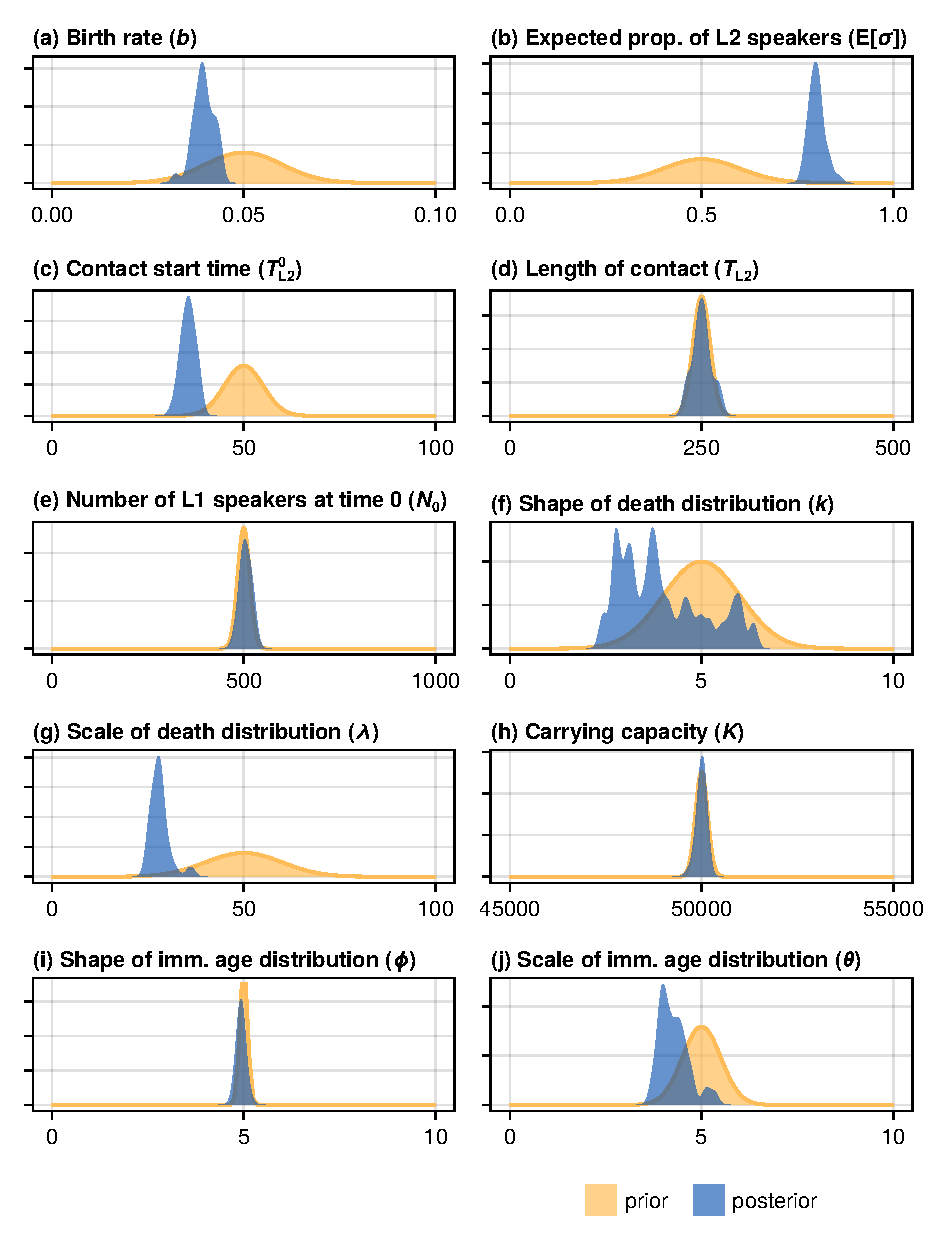
\includegraphics[width=1\textwidth]{figures/ch5/abc-APS.pdf}
\caption{Parameter estimation for Afro-Peruvian Spanish using
Approximate Bayesian Computation.}\label{fig:abc-aps}
}
\end{figure}

\begin{figure}
\hypertarget{fig:abc-afrikaans}{%
\centering
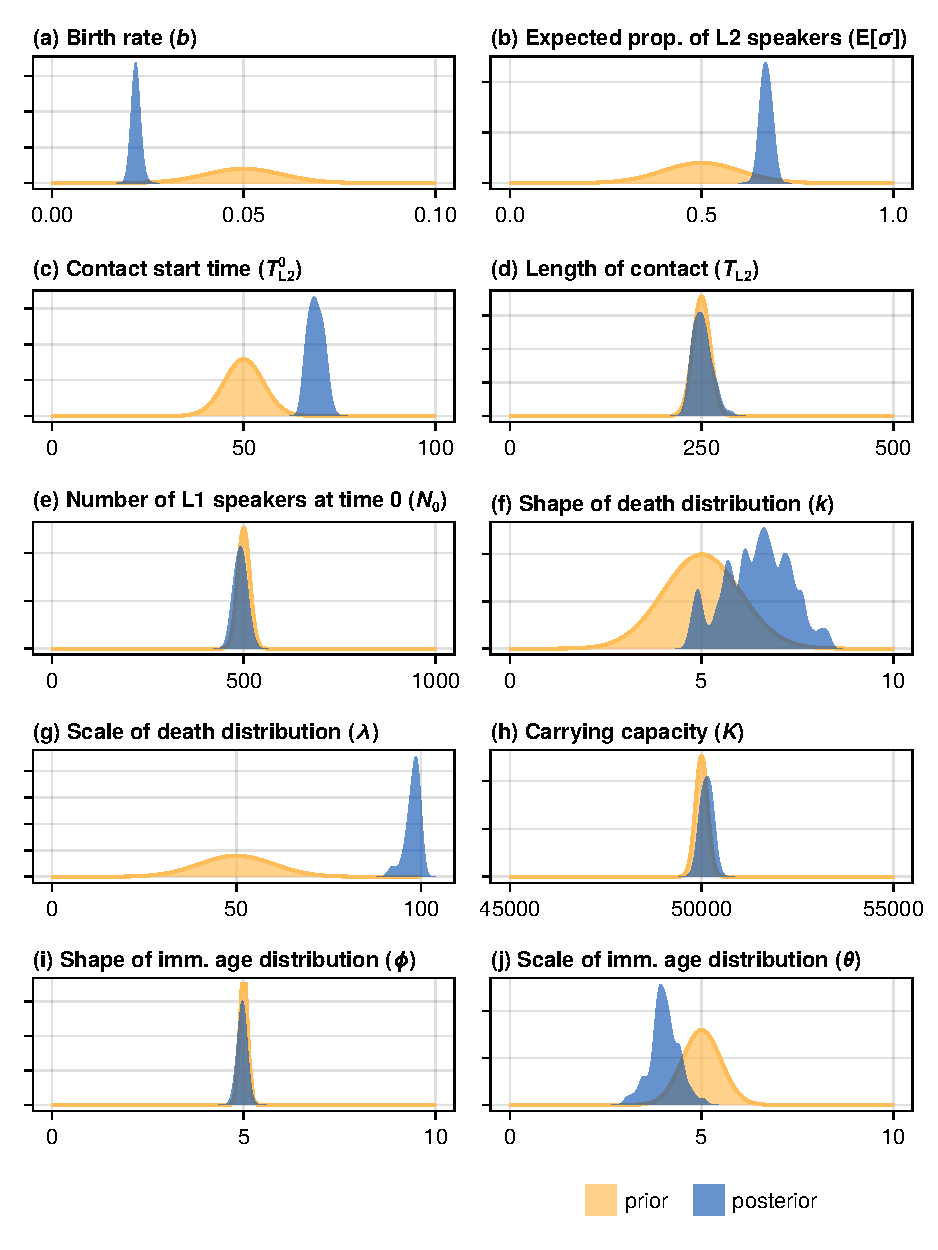
\includegraphics[width=1\textwidth]{figures/ch5/abc-Afrikaans.pdf}
\caption{Parameter estimation for Afrikaans using Approximate Bayesian
Computation.}\label{fig:abc-afrikaans}
}
\end{figure}

Next, 10 combinations of model parameters were sampled from the
posterior distributions to obtain simulations of each case study. These
sociodynamic parameters were combined with linguistic parameters:
\(a_1\) and \(a_2\), the advantages of the competing grammars, and
\(d\), the amount of L2-difficulty on grammar \(G_1\). For the advantage
parameters, estimates exist: as mentioned above, we have \(a_1 = 0.7\)
and \(a_2 = 0.05\) in the case of APS by the method of
\textcite{SimEtAl2019}. In the case of Afrikaans,
\textcite{Kauhanen2022} takes \(a_1 = a_2\) on the grounds that, Dutch
being a non-null subject language, the subject of the sentence can be
inferred even when verbal inflection is eroded. For the L2-difficulty
parameter \(d\), no estimates currently exist, and so we are forced to
sweep over this parameter, observing how variation in \(d\) affects the
model outcomes.

Figure \ref{fig:optimized-simulations} visualizes the mean value of
\(W_1\), the weight on the L2-difficult grammar \(G_1\), for each year
from the beginning of the simulation up to present day. Each panel of
the figure contains 150 curves, corresponding to five independent
simulations for three different values of the L2-difficulty parameter
\(d\) for each of the ten posterior samples.

\begin{figure}
\hypertarget{fig:optimized-simulations}{%
\centering
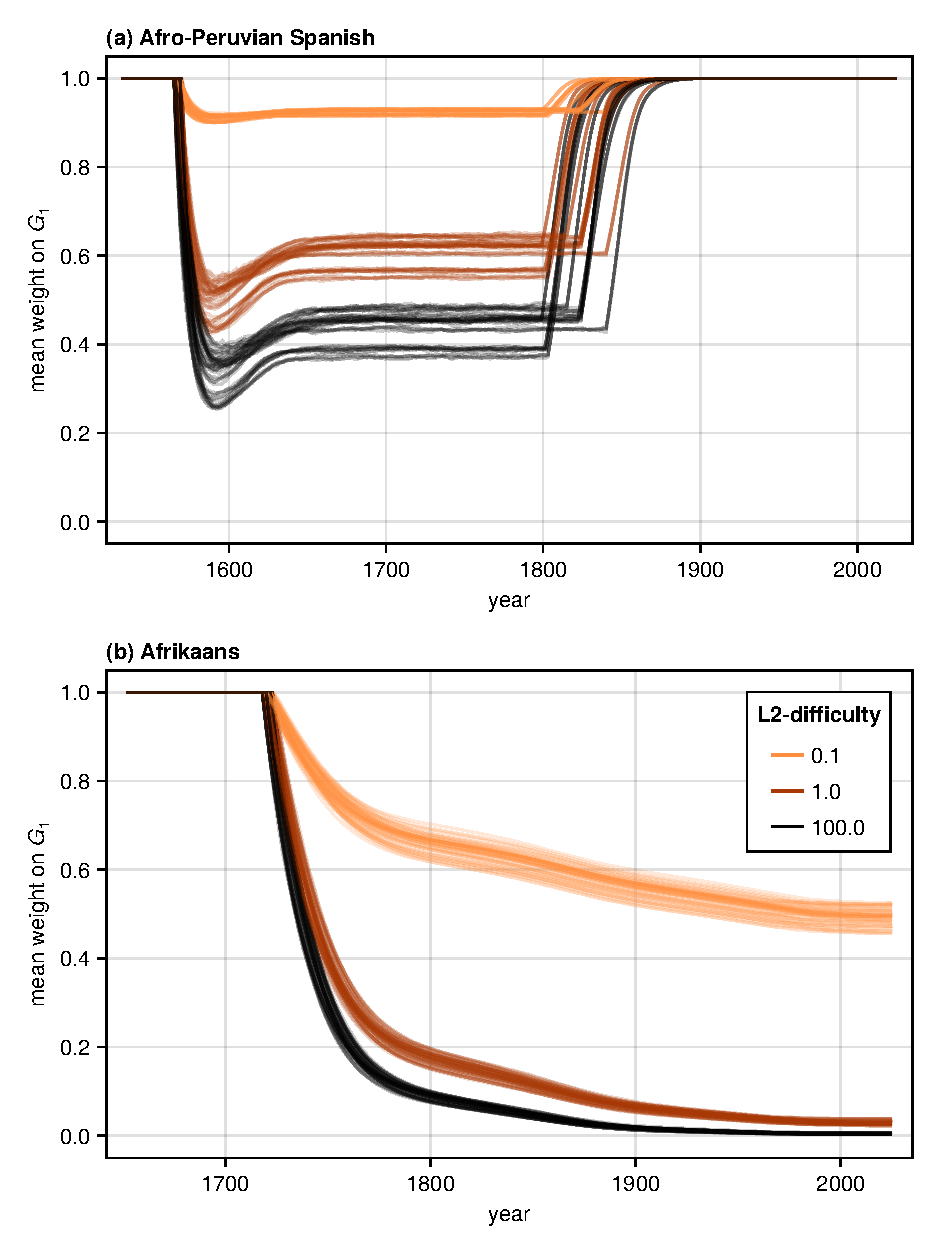
\includegraphics[width=1\textwidth]{figures/ch5/optimized-simulations.pdf}
\caption{Simulations of Afrikaans and Afro-Peruvian Spanish with
simulation parameters sampled from the posterior distributions of the
sociodynamic parameters found using Approximate Bayesian Computation
(Figures
\ref{fig:abc-aps}--\ref{fig:abc-afrikaans}).}\label{fig:optimized-simulations}
}
\end{figure}

For Afro-Peruvian Spanish, the simulation outcomes are consistent with
both the empirical reality and the deterministic result from
\textcite{Kauhanen2022}. Full simplification is never attained, no
matter how large the L2-difficulty \(d\). In all simulation runs,
moreover, once L2 learning is removed, the representation of the
L2-difficult grammar \(G_1\) returns back to full usage, replicating the
observation that younger speakers of APS are reverting back to using a
consistent null subject grammar \autocite{Ses2014}.

For Afrikaans, the simulation results are also roughly of the right
shape. For sufficiently high L2-difficulties, full simplification is
predicted by the 20th century. For very low L2-difficulties,
simplification takes so long that the process may in fact be halted, if
the supply of L2 learners is cut off before full simplification has been
attained.

\hypertarget{sec:discussion}{%
\section{Conclusion}\label{sec:discussion}}

This chapter has taken up the mathematical model of contact-induced
change proposed in \textcite{Kauhanen2022} and implemented the model in
a series of fairly realistic agent-based simulations. The simulations
involved finite (rather than infinite) populations, local (as opposed to
well-mixing) interaction patterns and finite (as opposed to eternal)
lifetimes for individual speakers. The central result of
\textcite{Kauhanen2022} -- the existence and location of a bifurcation
threshold involving the proportion of L2 learners -- was confirmed in
these finite simulations. In addition to systematic sweeps over the
model's parameter space, the two case studies of \textcite{Kauhanen2022}
were revisited in detail, with the population-dynamic model parameters
optimized with respect to historical demographic data.

These simulations have, however, only scratched the surface. In the
current implementation, the model involves 18 parameters which are for
the most part free to vary independently of each other. Although some
interesting parameter interactions were mentioned above -- such as
between lattice aspect ratio and L2-difficulty or the length of the
immigration period -- these interactions await further, more systematic
study. On the other hand, it would be possible to break away from the
current implementation, to explore other mechanisms of population
dynamics. For instance, the model can readibly be implemented on
arbitrary interaction networks rather than the simple lattice setup here
assumed. This opens up a line of investigation -- the intersection of
language dynamics and network science -- which only a handful of studies
have explored so far
\autocites[e.g.][]{KeGonWan2008,FagEtal2010,Kau2017,Josserand2021}.

\hypertarget{appendix-a-population-dynamics}{%
\section*{Appendix A: Population
dynamics}\label{appendix-a-population-dynamics}}
\addcontentsline{toc}{section}{Appendix A: Population dynamics}

The purpose of this appendix is to prove that, given the simulation
setup assumed above, the expected proportion of L2 learners in the
population is completely determined by the birth and immigration rates
\(b\) and \(m\): \[
\textnormal{E}[\sigma] = \frac{m}{b + m}.
\] More precisely, this is the asymptotic value of
\(\textnormal{E}[\sigma]\) if L2 learning is allowed to continue
indefinitely. In practice, in the simulations conducted in this chapter,
this number describes the peak proportion of L2 learners attained during
the \(T_\textnormal{L2}\) simulation steps when L2 learning occurs
(cf.~Figure \ref{fig:ts}).

Let \(X\) and \(Y\) refer to the numbers of L1 and L2 learners in the
population, respectively, at some given simulation step. Moreover, let
\(X'\) and \(Y'\) refer to these numbers at the immediately following
simulation step. Let \(B\) refer to the number of L1 learners born at a
given step, and let \(M\) refer to the number of L2 learners immigrated.
With the assumptions made in the main text, we have
\(B \sim \textnormal{Bin}(\lfloor N(1 - N/K) \rfloor^+, b)\), where
\(N = X+Y\) is the total population size, \(K\) is a constant (the
carrying capacity), and \(\lfloor a \rfloor^+ = \lfloor a \rfloor\) if
\(a > 0\) and \(\lfloor a \rfloor^+ = 0\) otherwise. Similarly,
\(M \sim \textnormal{Bin}(\lfloor N(1 - N/K) \rfloor^+, m)\).

The expected numbers of L1 and L2 learners after one iteration are thus
\[
\left\{
\begin{aligned}
\textnormal{E}[X'] &= \textnormal{E}[X] + \textnormal{E}[B] - \mu \textnormal{E}[X] \\
\textnormal{E}[Y'] &= \textnormal{E}[Y] + \textnormal{E}[M] - \mu \textnormal{E}[Y]
\end{aligned}
\right.
\] where \(\mu\) is a death rate (the exact value of this parameter will
depend on the parameterization of the Weibull distribution assumed in
the main text). The expected change between two consecutive steps is
thus \[
\left\{
\begin{aligned}
\textnormal{E}[X' - X] &= \textnormal{E}[B] - \mu \textnormal{E}[X] \\
\textnormal{E}[Y' - Y] &= \textnormal{E}[M] - \mu \textnormal{E}[Y]
\end{aligned}
\right.
\] Given that \(B\) and \(M\) are binomially distributed, the following
holds: \[
\left\{
\begin{aligned}
\textnormal{E}[X' - X] &= b \lfloor N(1 - N/K) \rfloor^+ - \mu \textnormal{E}[X] \\
\textnormal{E}[Y' - Y] &= m \lfloor N(1 - N/K) \rfloor^+ - \mu \textnormal{E}[Y]
\end{aligned}
\right.
\] Approximately, we have \[
\left\{
\begin{aligned}
\textnormal{E}[X' - X] &\approx b N(1 - N/K) - \mu \textnormal{E}[X] \\
\textnormal{E}[Y' - Y] &\approx m N(1 - N/K) - \mu \textnormal{E}[Y]
\end{aligned}
\right.
\] At equilibrium, one has \(\E [Y' - Y] = 0\) and so \[
m N(1 - N/K) = \mu \E [Y].
\] Taking expectations on both sides and dividing \(m\) onto the right
hand side, \[
\E [N] - \E [N]^2/K = \frac{\mu}{m} \E [Y].
\] Dividing both sides by \(\E [N]\) we obtain \[
1 - \E [N]/K = \frac{\mu}{m} \E [\sigma],
\] from which \begin{equation}
\E [\sigma] = \frac{m}{\mu} (1 - \E [N]/K).
\label{eq:sigma1}\end{equation} Carrying out the same exercise starting
from \(\E [X' - X] = 0\), one obtains \begin{equation}
\E [\sigma] = 1 - \frac{b}{\mu} (1 - \E [N]/K).
\label{eq:sigma2}\end{equation} Equating (\ref{eq:sigma1}) and
(\ref{eq:sigma2}) allows us to solve for \(\E [N] = \E [X + Y]\), the
expected total population size at equilibrium: \[
\E [N] = K\left(1 - \frac{\mu}{b + m} \right).
\] Substituting this back to (\ref{eq:sigma1}) finally gives us \[
\E [\sigma] = \frac{m}{\mu} \left(1 - \left(1 - \frac{\mu}{b + m}\right)\right) = \frac{m}{\mu} \cdot \frac{\mu}{b + m} = \frac{m}{b + m}
\] as desired.

Thus, in order to obtain a desired L2 learner proportion \(\sigma\)
given a fixed birth rate \(b\), we need to select the immigration rate
\(m\) such that \[
m = \frac{\sigma}{1 - \sigma} b.
\]

\hypertarget{appendix-b-parameter-estimation}{%
\section*{Appendix B: Parameter
estimation}\label{appendix-b-parameter-estimation}}
\addcontentsline{toc}{section}{Appendix B: Parameter estimation}

To estimate population-dynamical parameters for Afro-Peruvian Spanish
and Afrikaans, Approximate Bayesian Computation Sequential Monte Carlo
(ABC-SMC) \autocite{Toni_etal_2009,Sunnaker_etal_2013} with Differential
Evolution (DE) moves \autocite{StornPrice1997,DasSuganthan2011} was
used, as implemented in the ABCdeZ.jl package of the Julia programming
language \autocite{Julia}. The distance function between model
prediction and empirical data is given by \[
\mae (\vec{\pi}) = \frac{1}{|\mathcal{T}|} \sum_{t \in \mathcal{T}} \left|\ O_\textnormal{L1}(t) - P_\textnormal{L1}(t, \vec{\pi})\ \right| + \frac{1}{|\mathcal{T}|} \sum_{t \in \mathcal{T}} \left|\ O_\textnormal{L2}(t) - P_\textnormal{L2}(t, \vec{\pi}) \ \right|,
\] i.e.~by the mean absolute error (this has the straightforward
interpretation of being the average per-year error in total population
size between model and data). Here, \(\mathcal{T}\) denotes the set of
time points in the data (i.e.~the years for which demographic data is
available), \(O_\textnormal{L1}(t)\) denotes the empirical (observed)
number of L1 speakers at time \(t\), \(P_\textnormal{L1}(t, \vec{\pi})\)
denotes the modelled (predicted) number of L1 speakers at time \(t\),
given parameter vector \(\vec{\pi}\), and so on. In respect of the
empirical demographic data, I take all Europeans to be L1 speakers and
all non-Europeans to be L2 speakers (at least initially, i.e.~at the
time they are introduced into the population). This constitutes an
idealization, of course, but in the absence of further empirical
information it is difficult to see how one might proceed otherwise.

\begin{table}
\caption{Prior distributions of model parameters for ABC-SMC. `TrNormal' refers to a normal distribution truncated to the interval specified.}\label{tbl:optimizebounds}
\begin{tabular}{lcl}
\toprule
Parameter & Symbol & Prior\\
\midrule
Birth rate & $b$ & $\textnormal{TrNormal} (0.05, 0.01); [0, 1]$\\
Expected proportion of L2 learners & $\textnormal{E}[\sigma]$ & $\textnormal{TrNormal} (0.5, 0.1); [0, 1]$\\
Length of immigration period & $T_\textnormal{L2}$ & $\textnormal{Bin} (500, 0.5)$\\
Shape of immigration age distribution & $\phi$ & $\textnormal{TrNormal} (5, 0.1); [0, 10]$\\
Scale of immigration age distribution & $\theta$ & $\textnormal{TrNormal} (5, 0.5); [0, 10]$\\
Number of L1 speakers at time 0 & $N_0$ & $\textnormal{Bin} (1000, 0.5)$\\
Shape parameter of death distribution & $k$ & $\textnormal{TrNormal} (5, 1); [0, 10]$\\
Scale parameter of death distribution & $\lambda$ & $\textnormal{TrNormal} (50, 10); [0, 100]$\\
Population carrying capacity & $K$ & $\textnormal{Bin} (10^5, 0.5)$\\
Language contact start time & $T_\textnormal{L2}^0$ & $\textnormal{Bin} (100, 0.5)$\\
\bottomrule
\end{tabular}
\end{table}

The prior distributions assumed for the model parameters are indicated
in Table \ref{tbl:optimizebounds}. The procedure was continued until
\(\mae (\vec{\pi})\) stabilized i.e.~showed no more improvement. For
Afro-Peruvian Spanish, the summary statistic stabilized at
\(\mae(\vec{\pi}) = 1022.75\); for Afrikaans, the eventual value was
\(\mae(\vec{\pi}) = 3405.13\).

\section*{Abbreviations}

\begin{tabularx}{.45\textwidth}{lQ}
ABC & Approximate Bayesian Computation \\
APS & Afro-Peruvian Spanish \\
DE & Differential Evolution \\
\end{tabularx}
\begin{tabularx}{.45\textwidth}{lQ}
L1 & First language \\
L2 & Second language \\
MAE & Mean Absolute Error \\
SMC & Sequential Monte Carlo
\end{tabularx}

\hypertarget{acknowledgements}{%
\section*{Acknowledgements}\label{acknowledgements}}
\addcontentsline{toc}{section}{Acknowledgements}

The work presented here received funding from the European Research
Council (ERC) under the European Union's Horizon 2020 research and
innovation programme (grant agreement no. 851423). I am grateful to
Frederik Hartmann, Gemma Hunter McCarley, Raquel Montero, Molly Rolf and
George Walkden for their many helpful comments; any remaining errors
are, naturally, my sole responsibility.
